\documentclass[oneside,english]{amsbook}
\usepackage{lmodern}
\renewcommand{\sfdefault}{lmss}
\renewcommand{\ttdefault}{lmtt}
\renewcommand{\familydefault}{\rmdefault}
\usepackage[T1]{fontenc}
\usepackage[latin9]{inputenc}
\usepackage{amsthm}
\usepackage{amssymb}
\usepackage{esint}
\usepackage[all]{xy}

\makeatletter
%%%%%%%%%%%%%%%%%%%%%%%%%%%%%% Textclass specific LaTeX commands.
\numberwithin{section}{chapter}
\numberwithin{equation}{section}
\numberwithin{figure}{section}
\theoremstyle{plain}
\newtheorem{thm}{\protect\theoremname}
  \theoremstyle{definition}
  \newtheorem{defn}[thm]{\protect\definitionname}
  \theoremstyle{remark}
  \newtheorem*{rem*}{\protect\remarkname}
  \theoremstyle{definition}
  \newtheorem*{example*}{\protect\examplename}
 \theoremstyle{definition}
 \newtheorem*{defn*}{\protect\definitionname}
  \theoremstyle{plain}
  \newtheorem*{cor*}{\protect\corollaryname}

\makeatother

\usepackage{babel}
  \providecommand{\corollaryname}{Corollary}
  \providecommand{\definitionname}{Definition}
  \providecommand{\examplename}{Example}
  \providecommand{\remarkname}{Remark}
\providecommand{\theoremname}{Theorem}

\begin{document}

\title{Hitchin Systems Seminar}

\maketitle
\tableofcontents{}


\chapter{Introduction}

This course studies the Hitchin system from different perspectives and in various settings.

Hitchin studied a limiting form of the self-dual equations of Yang-Mills theory in four dimensions,
imposing invariance under two of the dimensions.  The resulting equations were found to be
conformally invariant with respect to the remaining two directions, so had a natural formulation
as equations on a Riemann surface.  The Hitchin moduli space, or moduli space of Higgs bundles,
will be defined as the space of solutions modulo gauge transformations.

Several basic properties of the space of solutions emerged.  First, the equations could be
interpreted formally as hyperkahler moment map equations for the compact gauge Group action
on the infinite-dimensional space of connections.  Since we quotient solutions by gauge
transformations, this means we have an interpretation of the Hithchin moduli space as a hyperkahler
quotient.  Thus it should inherit a hyperkaher structure.  Of the three independent complex structures,
the one most amenable to algebraic geometry is the one inherited from the complex
structue on the Riemann surface, $C$.  In that setting, the Hitchin moduli space has an
interpretation as stable Higgs pairs, i.e. pairs $(V,\varphi)$, where $V$ is a rank-$n$ holomorphic
vector bundle over $C$, and $\varphi\in \Gamma(End(V)\otimes K_C)$ is a holomorphic $n\times n$
matrix-valued one-form.  Stability requires that all $\varphi$-invariant sub-bundles have lesser slope
than $V$.  Finally, solutions are taken modulo holomorphic isomorphism of vector bundles.

Another structure which emerges is that of an algebraically completely integrable system.
Recall first that a complete integrable system on a symplectic manifold (``phase space'') is a
maximal set of Poisson-commuting proper functions (``Hamiltonians").  Specifying the values
of these conserved quantities gives a common level set which is a Lagrangian torus.
This gives another definition:  a fibration by Lagrangian tori to a base manifold where the
Hamiltonians take their values.  The fiber map for the Hitchin space is defined by all the
invariant polynomials $Tr\varphi^k$.

Local study....

\input{2-Definitions-Peng.tex}


\chapter{Symplectic Quotients in Finite and Infinite Dimensions}

%!TEX root = HitchinSystems.tex

\chapter{Hyperk\"ahler Quotients and Integrable Systems}


\newcommand{\bbR}{\mathbb{R}}
\newcommand{\bbC}{\mathbb{C}}
\newcommand{\bbZ}{\mathbb{Z}}
\newcommand{\bbA}{\mathbb{A}}
\newcommand{\bbP}{\mathbb{P}}
\newcommand{\bbF}{\mathbb{F}}
\newcommand{\ad}[0]{\mathrm{ad}\,}
\newcommand{\Mbar}[0]{\overline{\mathcal{M}}}








\section*{Introduction}
The objects of interest to us are as follows. Let $P\to X$ be a principal $G$-bundle over $X$ where $G$ is a compact Lie group. We may consider pairs $(A,\Phi)$ where $A$ is a unitary connection on $P$ and $\Phi\in \Omega^{1,0}(X;\ad P\otimes \bbC)$. By looking at 4-dimensional Yang Mills theory dimensionally reduced to $X$, we may become interested in such pairs which satisfy the self-duality equations 
\begin{align}
 &F_A =- [\Phi,\Phi^*]\\
 &\bar{\partial}_A\Phi = 0
\end{align}
where $F$ is the curvature of $A$ and $\bar{\partial}_A$ is the anti-holomorphic part of the covariant derivative with respect to $A$ (we will probably abbreviate at least the former by writing simply $F$). We will denote the space of pairs satisfying the self-duality equations by $\Mbar$. Finally, we would like to study the quotient of $\Mbar$ by the action of the group of gauge transformations, denoted $\mathscr{G}$. Elements of $\mathscr{G}$ are functions on $M$ with values in the adjoint representation of $P$, i.e. $\psi\in \Omega^0(X;\ad P)$, and the action of $\mathscr{G}$ on a pair $(A,\Phi)$ is given by
\begin{align*}
  &A\mapsto \psi d \psi^{-1} + \psi A \psi^{-1} = \psi d_A \psi^{-1}\\
  &\Phi \mapsto \psi \Phi \psi^{-1} 
\end{align*}
where $d_A$ is the covariant derivative with respect to $A$ (showing that gauge transformations preserve self-duality is a nice exercise). We will denote this quotient by $\mathcal{M}$. The goal of this talk is to show that $\mathcal{M}$ can be realized as a Hyperk\"ahler quotient.  

\section{Symplectic Reduction and K\"ahler Quotients}
\subsection{Rapid Review of Symplectic Reduction}
Hyperk\"ahler quotients can be thought of as an extension of symplectic reduction, so we will briefly review the main ingredients to the symplectic reduction procedure here. The main idea is: given a manifold with some structure (a symplectic form) and a group action which respects that structure, we would like to quotient by the group action in such a way that the resulting object is a manifold with the same type of structure. This will be the main recurring theme as we proceed. 

Let $(M,\omega)$ be a symplectic manifold, which, to avoid difficulty, we take to be finite dimensional.\footnote{The case we care about will not be finite-dimensional, but we will see that the statements made here will still hold in this case.} Now, let $G$ be a connected Lie group which acts on $M$ by symplectomorphisms. We say this group action is Hamiltonian if ther exists a map $\mu^*: \mathfrak{g}\to C^\infty(M)$ such that:
\begin{enumerate}
  \item The map $\mathfrak{g}\to \mathfrak{X}(M)$ which sends $\xi\mapsto X_\xi$ has image contained in the set of Hamiltonian vector fields. Moreover, for any $\xi\in \mathfrak{g}$, $\mu^*(\xi)$ is the Hamiltonian function for $X_\xi$, i.e. 
\begin{equation*}
  d(\mu^*(\xi)) = \iota_{X_\xi}\omega.
\end{equation*}
  \item $\mu$ is a Lie algebra anti-homomorphism, i.e. 
\begin{equation*}
  \mu^*([\xi,\eta]) = - \{\mu^*(\xi),\mu^*(\eta)\}.
\end{equation*}
\end{enumerate}
In this case, we may define the moment map\footnote{$\mu^*$ is sometimes called the comomentum map.} $\mu: M\to\mathfrak{g}^*$ by $\langle \mu(x),\xi\rangle = (\mu^*(\xi))(x)$. Condition (2) above is equivalent to saying that $\mu$ is $G$-equivariant with respect to the coadjoint action on $\mathfrak{g}^*$, which means that the set $\mu^{-1}(0)\subset M$ is invariant under the $G$-action. As long as 0 is a regular value of $\mu$, this will actually be an embedded submanifold of $M$. If the $G$-action is free on $\mu^{-1}(0)$, then the quotient $\mu^{-1}(0)/G$ will also be a manifold which we denote by $M\sslash G$. In this case, we have the following theorem:
\begin{thm}[Marsden-Weinstein]
  If $(M\omega)$, $G$, and $\mu$ are as above and $M\sslash G := \mu^{-1}(0)/G$ is a manifold, then $M\sslash G$ is symplectic with symplectic form $\omega'$ uniquely defined by the property that $\pi^*\omega' = i^*\omega$ where $i:\mu^{-1}(0)\to M$ and $\pi: \mu^{-1}(0)\to M\sslash G$ are the inclusion and quotient maps respectively. 
\end{thm}
\subsection{Quotients and K\"ahler Structure}
First, we recall the definition of a K\"ahler manifold. We say a manifold $M$ endowed with a metric $g$, complex structure $\mathbf{J}$, and symplectic form $\omega$ is K\"ahler if these three structures are compatible. This may be defined in a variety of ways. One possibility is to require $\mathbf{J}$ to be covariantly constant with respect to the Levi-Civita connection induced by $g$ and then to define $\omega(X,Y) = g(\mathbf{J}X,Y)$ for vector fields $X$ and $Y$.\footnote{Actually, by choosing any two of the metric, complex structure, and symplectic form and requiring that these are compatible in the appropriate sense, we may construct the third structure in a compatible way.} We can also see that the structure group of a K\"ahler manifold has been reduced to $U(n)$, where $2n$ is the real dimension of the manifold, since the metric, complex structure, and symplectic form reduce the structure group to $\mathrm{O}(2n)$, $\mathrm{GL}(n,\bbC)$, and $\mathrm{Sp}(2n,\mathbb{R})$ respectively. 

Since K\"ahler manifolds are symplectic manifolds, we may ask whether the process of symplectic reduction preserves the K\"ahler structure. To answer this, we first consider how a metric may descend to a quotient manifold. Let $(M,g)$ be a Riemannian manifold and let $G$ be a connected Lie group which acts on $M$ by isometries. We will require that $M/G$ comes with a natural manifold structure, in particular the $G$-action must be free. Then, the space $M$ has the structure of a principal $G$-bundle over $M/G$. At any point $x\in M$, the vertical subspace of the tangent space at $x$, $V_x\subset T_xM$, is isomorphic to $\mathfrak{g}$. Moreover, since the $G$-action on $M$ is free, there are non-vanishing vector fields which generate $V_x$ at each point. Then, the operation of orthogonal projection onto $V_x$ at each point defines a one form, $\theta$, with values in $\mathfrak{g}$ which transforms under the adjoint representation of $G$. $\theta$ defines a connection on $M$, i.e. a distribution of horizontal subspaces $H_x\subset T_xM$ complementary to $V_x$. Then, for any vector fields $X,Y$ on $M/G$, we can use the connection to lift these to horizontal vector fields $\tilde{X},\tilde{Y}$ on $M$. We see that the metric $h(X,Y) = g(\tilde{X},\tilde{Y})$ is well defined using this choice of (orthogonal) horizontal lift since $g$ is invariant under the $G$-action. 

Now, we can answer our question about whether symplectic reduction preserves K\"ahler structure. 
\begin{prop}
  Let $(M,g,\mathbf{J},\omega)$ be a K\"ahler mainfold and let $G$ be a connected Lie group with a Hamiltonian action on $(M,\omega)$ which preserves the metric (and hence complex structure). Also, we require that $M\sslash G$ has a natural manifold structure. Then the naturally induced metric $g'$ on $M\sslash G$ gives $M\sslash G$ the structure of a K\"ahler manifold. 
\end{prop}
\begin{proof}[Sketch of proof]
  Let $N = \mu^{-1}(0)$ so that $N/G = m\sslash G$. Then $TN$ is a sub-bundle of $TM$ and we can further restrict to the horizontal sub-bundle $H\subset TN$ defined by the connection on $N\to N/G$ in the manner discussed above. The Levi-Civita connection with respect to $g'$ on $T(N/G)$ will pull back to a $G$-invariant connection on $H\to N$. We will use the fact that this connection on $H$ is given by orthogonal projection of the Levi-Civita connection of $g\big|_N$ on $TM\big|_N$ to $H$ (for an explanation, see \cite{HKLR}). Now, let $x\in N$. The complement of $T_xN\subset T_xM$ is spanned by the vectors $(\mathrm{grad}\,\mu^{\xi_i})_x$ for $\xi_i$ a basis of $\mathfrak{g}$ (here we have used the notation $\mu^{\xi_i} := \mu^*(\xi_i)$) and the complement of $H$ in $TN$ is spanned by the vertical vectors $k_i$ which are associated to the basis $\xi_i$ of $\mathfrak{g}$. By definition, 
\begin{equation*}
  g(\mathrm{grad}\,\mu^{\xi},Y) = d\mu^\xi(Y) = \omega(X_\xi,Y) = g(\mathbf{J}X_\xi,Y)
\end{equation*}
for any vector field $Y$ on $M$, and so $\mathrm{grad}\,\mu^\xi = \mathbf{J}X_\xi$. This shows that the vector space spanned by $k_i$ and $(\mathrm{grad}\,\mu^{\xi_i})_x$ is a complex vector space. Moreover, since the basis $\{k_1,...,k_{\dim G}\}$ can be extended to a global frame for the vertical sub-bundle $V\subset TN$, we see that the sub-bundle complementary to $H$ over $N$ is a complex sub-bundle, hence $H$ is as well. This means that $\mathbf{J}\big|_N$ commutes with orthogonal projection onto $H$, and since $\mathbf{J}$ is compatible with $g$, this implies that $\mathbf{J}\big|_N$ is covariantly constant with respect to the orthogonal projection of the Levi-Civita connection of $g\big|_N$ on $TM\big|_N$ to $H$. Since this is just the pull back of the Levi-Civita connection of $g'$ on $T(N/G)$ to $N$ and $\mathbf{J}$ was assumed to be $G$-invariant, we see that $\mathbf{J}$ descends to a complex structure on $N/G$ which is compatible with the induced metric $g'$. 
\end{proof}
\section{Hyperk\"ahler Quotients}
\subsection{Rapid Review of Hyperk\"ahler Manifolds}
Hyperk\"ahler structure can be thought of as a ``quaternionic'' extension of K\"ahler structure. In particular, we say that a Riemannian manifold $(M,g)$ is Hyperk\"ahler if it is equipped with three complex structures $\mathbf{I}$, $\mathbf{J}$, and $\mathbf{K}$, each of which are covariantly constant, and which satisfy quaternionic algebraic relations (i.e. $\mathbf{I}^2 = -1$, $\mathbf{J}^2 = -1$, $\mathbf{K}^2 = -1$, $\mathbf{I}\mathbf{J} = \mathbf{K}$, etc.). As a result, the tangent space at each point becomes a quaternionic vector space and the structure group is reduced to $\mathrm{O}(4n)\cap \mathrm{GL}(n,\mathbb{H}) = \mathrm{Sp}(n)$. As in the K\"ahler case, each of these complex structures defines a symplectic form compatible with the metric: $\omega_1(X,Y) = g(\mathbf{I}X,Y)$, $\omega_2(X,Y) = g(\mathbf{J}X,Y)$, and $\omega_3(X,Y) = g(\mathbf{K}X,Y)$. This means that each triple $(g, \mathbf{I}, \omega_1)$ gives $M$ the structure of a K\"ahler manifold. 
\subsection{Quotients and Hyperk\"ahler Structure}
If $(M,g,\vec{\mathbf{I}},\vec{\omega})$ is a Hyperk\"ahler manifold and $G$ is a connected Lie group which acts on $M$ in a Hamiltonian manner with respect to each symplectic structure and preserves the metric, then we may consider the symplectic reduction of $M$ with respect to each of the three moment maps $\mu_1$, $\mu_2$, and $\mu_3$. From the section above, we see that each of these quotients will inherit a K\"ahler structure from $M$. Now, we would like to define a new type of quotient which inherits the Hyperk\"ahler structure from $M$. 

The key will be to consider one moment map
\begin{equation*}
  \mu: M\to \mathfrak{g}^*\otimes \mathbb{R}^3
\end{equation*}
defined by $\mu(x) = (\mu_1(x),\mu_2(x),\mu_3(x))$. Then, if 0 is a regular value of $\mu$, we see that $\mu^{-1}(0)$ is an embedded submanifold in $M$ which is invariant under the $G$-action. Furthermore, if the $G$-action is free on $\mu^{-1}(0)$, then the quotient $\mu^{-1}(0)/G$ will have a natural manifold structure. 
\begin{prop}
  If $(M,g,\vec{\mathbf{I}},\vec{\omega})$ and $G$ are as above, then the quotient $\mu^{-1}(0)/G$ with the inherited metric, complex structures, and symplectic forms is a Hyperk\"ahler manifold. 
\end{prop}
\begin{proof}
  We begin by defining the complex moment map
\begin{equation*}
  \mu_+ = \mu_2 + i\mu_3 : M \to \mathfrak{g}^*\otimes \bbC.
\end{equation*}
Then we see that $d\mu_+^\xi(Y) = \omega_2(X_\xi,Y) + i\omega_3(X_\xi,Y) = g(\mathbf{J}X_\xi,Y) + ig(\mathbf{K}X_\xi,Y)$ while $d\mu_+^\xi(\mathbf{I}Y) = \omega_2(\mathbf{J}X_\xi,\mathbf{I}Y) + i\omega_3(\mathbf{K}X_\xi,\mathbf{I}Y) = -g(\mathbf{K}X_\xi,Y) + ig(\mathbf{J}X_\xi,Y)$. Thus, $id\mu_+^\xi(Y) = d\mu_+^\xi(\mathbf{I}Y)$ for all vector fields $Y$ on $M$. Working in local holomorphic coordinates at any point in $M$, we may consider the vector fields $\frac{\partial}{\partial \bar{z}^i}$, which satisfy
\begin{equation*}
  \mathbf{I}\frac{\partial}{\partial \bar{z}^i} = -i \frac{\partial}{\partial \bar{z}^i}.
\end{equation*}
Then, plugging this into the result above gives
\begin{equation*}
  i\frac{\partial \mu^\xi_+}{\partial \bar{z}^i} = id\mu^\xi_+\left(\frac{\partial}{\partial \bar{z}^i}\right)=d\mu^\xi_+\left( \mathbf{I}\frac{\partial}{\partial \bar{z}^i}\right) = -i \frac{\partial \mu^\xi_+}{\partial \bar{z}^i}
\end{equation*}
so $\mu^\xi_+$ is a holomorphic function. Thus, as long as 0 is a regular value of $\mu_+$, we see that $\mu_+^{-1}(0)$ is an embedded complex submanifold of $M$ with respect to the complex structure $\mathbf{I}$. This means that $\mu_+^{-1}(0)$ is K\"ahler with its induced metric. Now, consider the $G$-action restricted to $\mu_+^{-1}(0)$. This still preserves the metric and the complex structure $\mathbf{I}$, and we can restrict the moment map $\mu_1$ to this submanifold, giving us a moment map for the $G$-action with respect to the restricted symplectic form $\omega_1$. Then, from the previous proposition, we see that $\mu_1^{-1}(0)\cap\mu_+^{-1}(0)/G$ is a K\"ahler manifold with the induced metric and complex structure. It follows that $\mu^{-1}(0)/G$ is K\"ahler with respect to $\mathbf{I}$ since $\mu_+^{-1}(0) = \mu_2^{-1}(0)\cap\mu_3^{-1}(0)$. Repeating this argument for $\mathbf{J}$ and $\mathbf{K}$ shows that each of these define a K\"ahler structure on $\mu^{-1}(0)/G$. 
\end{proof}
\subsection{Main Example}
Now we may relate these new definitions to the subject of interest to us: the self-duality equations and the moduli space $\mathcal{M}$. We begin by looking at the manifold consisting of pairs $(A,\Phi)$ as in the introduction (we will use Hiychin's notation for this manifold, denoting it by $\mathscr{A}\times \Omega$). The tangent space to this manifold at a point $(A,\Phi)$ is given by $\Omega^{0,1}(X;\ad P\otimes \bbC)\oplus \Omega^{1,0}(X;\ad P\otimes \bbC)$. We can define a symplectic structure on $\mathscr{A}\times \Omega$ as follows:
\begin{equation*}
  \omega((\Psi_1,\Phi_1),(\Psi_2 ,\Phi_2)) = \int_X \mathrm{Tr}(\Phi_2\Psi_1 - \Phi_1\Psi_2)
\end{equation*}
where $(\Psi_i,\Phi_i)\in \Omega^{0,1}(X;\ad P\otimes \bbC)\oplus \Omega^{1,0}(X;\ad P\otimes \bbC)$. $\omega$ is clearly non-degenerate. To see it is closed, we note that $\omega$ has constant coefficients in $(\Psi_i,\Phi_i)$ and that $\mathscr{A}\times \Omega$ is an affine space. 

Now, define the vector field $X = (\Psi_1,\Phi_1)$ on $\mathscr{A}\times \Omega$ by $\Psi_1 = \bar{\partial}_A\psi$ and $\Phi_1 = [\Phi,\psi]$ where $\psi\in \Omega^0(X;\ad P)$ is an infinitesimal gauge transformation. Moreover, since $\mathscr{A}\times \Omega$ is an affine space, we may consider the vector field $(\dot{A}^{0,1},\dot{\Phi})$ where $(A,\Phi)\in \mathscr{A}\times\Omega$. Then, we can compute
\begin{align*}
  (\iota_X\omega)(\dot{A}^{0,1},\dot{\Phi}) &= \int_X \mathrm{Tr}(-[\Phi,\psi]\dot{A}^{0,1} + \dot{\Phi}\bar{\partial}_A\psi) \\
&= \int_X \mathrm{Tr}(\psi[\dot{A}^{0,1},\Phi] + \bar{\partial}_A\dot{\Phi}\psi) \\
&= df(\dot{A}^{0,1},\dot{\Phi})
\end{align*}  
where $f = \int_X\mathrm{Tr}(\bar{\partial}_A\Phi\psi)$. Thus, for the complex symplectic form $\omega$, we have shown that the function $f$ is Hamiltonian with respect to the vector field $X$. Moreover, one can check that the assignment $\psi \mapsto f$ is equivariant with respect to the action of the group $\mathscr{G}$, so we see that $f$ defines a moment map for this action. We define $\omega_2$ and $\omega_3$ to be the real and imaginary parts of the symplectic form $\omega$, and $\mu_2$, $\mu_3$ to be the real and imaginary parts of the moment map $\mu$ defined by $f$. Furthermore, $\mathscr{A}\times\Omega$ comes with a natural K\"ahler metric defined by
\begin{equation*}
  g((\Psi,\Phi),(\Psi,\Phi)) = 2i\int_X\mathrm{Tr}(\Psi^*\Psi + \Phi\Phi^*)
\end{equation*}
where $(\Psi,\Phi)\in \Omega^{0,1}(X;\ad P\otimes \bbC)\oplus \Omega^{1,0}(X;\ad P\otimes \bbC)$. This defines a third symplectic form $\omega_1$ on $\mathscr{A}\times\Omega$. It turns out that all three of these symplectic forms are compatible with the metric $g$ and that together with $g$ they define a Hyperk\"ahler structure on $\mathscr{A}\times \Omega$ (see section 6 of \cite{H1}). Moreover, if we recall that the moment map associated to $\omega_1$ was defined by $\mu_1(A,\Phi) = F_A + [\Phi,\Phi^*]$, we see that requiring $\mu_1(A,\Phi) = 0$ is equivalent to the self-duality equation (1). Furthermore, we can see that requiring $\mu(A,\Phi) = \mu_2(A,\Phi) + i\mu_3(A,\Phi) = 0$ is equivalent to requiring $\bar{\partial}_A\Phi = 0$, which is exactly self-duality equation (2). Thus, the Hyperk\"ahler quotient $\mu^{-1}(0)/\mathscr{G}$ is exactly the moduli space of solutions $\mathcal{M}$. 

With this result in hand, we may hope that the result from the previous section tells us that $\mathcal{M}$ is a Hyperk\"ahler manifold. However, in this infinite-dimensional setting the result is a purely formal statement. Instead, it is possible to directly show that $\mathcal{M}$ has a Hyperk\"ahler structure. 
\begin{prop}
  Let $\mathscr{A}\times\Omega$ and $\mathscr{G}$ be as above. Then the Hyperk\"ahler quotient $\mu^{-1}(0)/\mathscr{G}$ inherits the structure of a Hyperk\"ahler manifold (assuming it has a manifold structure to begin with). 
\end{prop}
In the specific case \cite{H1} deals with, this result appears as Theorem 6.7. We will only go through the main points of the proof here. 
\begin{proof}[Rough sketch of proof]
  The result of Marsden and Weinstein tells us that each of the inherited symplectic structures on $\mu^{-1}(0)/\mathscr{G}$ is, in fact, closed and non-degenerate. Moreover, it is possible to show that each complex structure on $\mathscr{A}\times\Omega$ induces an almost complex structure on $\mu^{-1}(0)/\mathscr{G}$. Then, \cite{H1} shows that the integrability of the induced complex structures is implied as long as the corresponding symplectic forms are closed. Since we know this is the case, we obtain three complex structures on $\mu^{-1}(0)/\mathscr{G}$ each compatible with $g$. It is left to check that these complex structures satisfy the quaternionic algebraic relations. However, this must only be checked on each tangent space, and this local property follows directly from the construction of these complex structures from the complex structures on 
$\mathscr{A}\times\Omega$. 
\end{proof}









\chapter{Stability and the Narasimhan-Seshadri Theorem}

\input{6-Teichmueller-Theory-Linhui.tex}

%% Matthew's talk #1
\chapter{Construction of the Hitchin Moduli Space}


This talk closely follows \cite{H1}. In this chapter, it is shown
that the Hitchin moduli space $\mathcal{M}_{H}$ is a smooth manifold
of dimension $12(g-1)$. We also prove that $\mathcal{M}_{H}$ is
equipped with a complete hyperkahler metric.


\section{Definitions}

Let $M$ be a Riemannian surface, $P\rightarrow M$ a principal $G=SO\left(3\right)$-bundle,
$V$ the associated rank 2 vector bundle, and $\mathcal{G}$ the group
of gauge transformations ($\mathcal{G}=Map\left(M,G\right)$). Recall
that for a connection $A$ on $P$ and $\Phi\in\Omega_{M}^{1,0}\left(adP\otimes\mathbb{C}\right)$,
the self-dual equations are
\begin{align*}
\tag{\ensuremath{\star}}F_{A}+\left[\Phi,\Phi^{*}\right] & =0,\\
\overline{\partial_{A}}\Phi & =0
\end{align*}


For a connection $A$, $u\in\mathcal{G}$ acts by
\[
u\left(A\right)=uAu^{-1}-\left(du\right)u^{-1}
\]
(where the covariant derivative is $\nabla_{A}=d+A\wedge$, i.e.,
\[
\nabla_{u\left(A\right)}s=u\nabla_{A}\left(u^{-1}s\right)
\]
for a section $s$ of $V$.

For $\Phi\in\Omega_{M}^{1,0}\left(adP\otimes\mathbb{C}\right)$, $u$
acts by
\[
u\left(\Phi\right)=u\Phi u^{-1},
\]
where we regard $adP\otimes\mathbb{C}$ as the bundle of trace-zero
endomorphisms of $V$.
\begin{defn}
The Hitchin moduli space is
\[
\mathcal{M}_{H}:=\left\{ \mbox{solutions to (}\star\mbox{)}\right\} /\mathcal{G}.
\]
\end{defn}
\begin{description}
\item [{Goal}] To learn about the geometry and topology of $\mathcal{M}_{H}$.
\end{description}

\section{Summary of results}

Let $V$ be a rank 2, odd degree vector bundle over a Riemannian surface
$M$. Then,
\begin{itemize}
\item $\mathcal{M}_{H}$ is a smooth manifold of dimension $12\left(g-1\right)$.
\item $\mathcal{M}_{H}$ has a natural metric.
\item $\mathcal{M}_{H}$'s metric is complete and hyperkahler (in fact,
$\mathcal{M}_{H}$ is a hyperkahler quotient).\end{itemize}
\begin{rem*}
$V$ has odd degree $\implies$ there are no reducible solutions to
$\left(\star\right)$ $\implies$ $\mathcal{G}$ acts freely on $\left(\star\right)$.
\end{rem*}

\section{$\mathcal{M}_{H}$ is a dimension $12\left(g-1\right)$ smooth manifold}

First, to get the expected dimension, we compute the dimension of
the tangent space to $\mathcal{M}_{H}$ at a regular point (i.e.,
one with trivial isotropy group).


\subsection{Idea of Proof}
\begin{itemize}
\item Linearize $(\star)$ to determine the expected dimension.
\item Let $\left(A\times\Omega\right)_{0}$ denote ``regular points,''
i.e., ones which are only fixed by the identity in $\mathcal{G}$
(those with trivial isotropy group). Then, exhibit $\mathcal{M}_{H}$
is a smooth submanifold of $\left(\mathcal{A}\times\Omega\right)_{0}/\mathcal{G}$
using the regular value theorem.
\end{itemize}

\subsection{Linearization of $(\star)$}

Let $\left(\dot{A},\dot{\Phi}\right)\in\Omega_{M}^{1}\left(adP\right)\oplus\Omega_{M}^{1,0}\left(adP\otimes\mathbb{C}\right)$.
To get the linearization of $(\star$), fix a base point $\left(A,\Phi\right)$
and look at
\[
\left.\frac{d}{dt}\right|_{t=0}\left(\star\right)\left(A+t\dot{A},\Phi+t\dot{\Phi}\right).
\]
Recalling that $F_{A}=dA+A\wedge A$, the first equation becomes
\[
d_{A}\dot{A}+\left[\dot{\Phi},\Phi^{*}\right]+\left[\Phi,\dot{\Phi}^{*}\right]=0,
\]
and the second is
\[
\overline{\partial_{A}}\dot{\Phi}+\dot{A}^{0,1}\wedge\Phi=0.
\]


$\left(\dot{A},\dot{\Phi}\right)$ arises from an infinitesimal gauge
transformation $\dot{\psi}\in\Omega_{M}^{0}\left(adP\right)$ if
\begin{align*}
\dot{A} & =d_{A}\dot{\psi}, & \dot{\Phi} & =\left[\Phi,\dot{\psi}\right].
\end{align*}
Let
\begin{eqnarray*}
d_{1}:\Omega_{M}^{0}\left(adP\right) & \longrightarrow & \Omega_{M}^{1}\left(adP\right)\oplus\Omega_{M}^{1,0}\left(adP\otimes\mathbb{C}\right)\\
\dot{\psi} & \mapsto & \left(d_{A}\dot{\psi},\left[\Phi,\dot{\psi}\right]\right)
\end{eqnarray*}
and
\begin{eqnarray*}
d_{2}:\Omega_{M}^{1}\left(adP\right)\oplus\Omega_{M}^{1,0}\left(adP\otimes\mathbb{C}\right) & \longrightarrow &
\Omega_{M}^{2}\left(adP\right)\oplus\Omega_{M}^{2}\left(adP\otimes\mathbb{C}\right)\\
\left(\dot{A},\dot{\Phi}\right) & \mapsto &
\left(d_{A}\dot{A}+\left[\dot{\Phi},\Phi^{*}\right]+\left[\Phi,\dot{\Phi}^{*}\right],\overline{\partial_{A}}\dot{\Phi}+\dot{A}^{0,1}\wedge\Phi\right).
\end{eqnarray*}
Then, $d_{1},d_{2}$ define an \emph{elliptic complex} with index
$3\left(2-2g\right)-6\left(g-1\right)=12\left(1-g\right)$. The Atiyah-Singer
index theorem then says that
\[
\dim H^{0}-\dim H^{1}+\dim H^{2}=12\left(1-g\right).
\]



\subsection{Elliptic Complexes}

Now, a short digression into elliptic complexes. Let $X$ be a manifold,
$\pi:T^{*}X\rightarrow X$ be projection onto the base, and $\left\{ E_{k}\rightarrow X\right\} $
a collection of vector bundles over $X$.
\begin{defn}
A chain complex
\[
\xymatrix{\cdots\ar[r] & \Gamma\left(E_{k-1}\right)\ar[r]^{P_{k-1}} & \Gamma\left(E_{k}\right)\ar[r]^{P_{k}} & \Gamma\left(E_{k+1}\right)\ar[r] & \cdots}
\]
is \textbf{elliptic} if the corresponding sequence of symbols
\[
\xymatrix{\cdots\ar[r] & \pi^{*}E_{k-1}\ar[r]^{\sigma\left(P_{k-1}\right)} & \pi^{*}E_{k}\ar[r]^{\sigma\left(P_{k}\right)} & \pi^{*}E_{k+1}\ar[r] & \cdots}
\]
is exact.\end{defn}
\begin{example*}
Let $P:E_{1}\rightarrow E_{2}$ be a differential operator. Then,
the complex
\[
\xymatrix{0\ar[r] & \Gamma\left(E_{1}\right)\ar[r]^{P} & \Gamma\left(E_{2}\right)\ar[r] & 0}
\]
is elliptic means that
\[
\xymatrix{0\ar[r] & \pi^{*}E_{1}\ar[r]^{\sigma\left(P\right)} & \pi^{*}E_{2}\ar[r] & 0}
\]
is exact, i.e., that $\sigma\left(P\right):\pi^{*}E_{1}\rightarrow\pi^{*}E_{2}$
is an isomorphism. Recall that this is the ``usual'' definition
of elliptic differential operator.
\end{example*}
Now, return to our elliptic complex.

\[
\xymatrix{\Omega_{M}^{0}\left(adP\right)\ar[r]^-{d_{1}} & \Omega_{M}^{1}\left(adP\right)\oplus\Omega_{M}^{1,0}\left(adP\otimes\mathbb{C}\right)\ar[r]^-{d_{2}} &
\Omega_{M}^{2}\left(adP\right)\oplus\Omega_{M}^{2}\left(adP\otimes\mathbb{C}\right)\\
\dot{\psi}\ar@{|->}[r] & \left(d_{A}\dot{\psi},\left[\Phi,\dot{\psi}\right]\right)\\
 & \left(\dot{A},\dot{\Phi}\right)\ar@{|->}[r] &
 \left(d_{A}\dot{A}+\left[\dot{\Phi},\Phi^{*}\right]+\left[\Phi,\dot{\Phi}^{*}\right],\overline{\partial_{A}}\dot{\Phi}+\dot{A}^{0,1}\wedge\Phi\right)
}
\]

By construction, we're interested in $H^{1}$ of this complex: $H^{0}=\ker d_{1}$
is the covariantly constant $\dot{\psi}$ which commute with $\Phi$.
These correspond to reducible solutions to $(\star$). So, if $H^{0}\neq0$,
then $\left(A,\Phi\right)$ is reducible. In fact, by considering
$d_{2}^{*}$, we can show that $H^{2}=0$ as well \cite{H1}. Hence,
\[
-\dim H^{1}=12\left(1-g\right),
\]
i.e., for a regular point $\left(A,\Phi\right)$,
\[
\boxed{\dim T_{\left(A,\Phi\right)}\mathcal{M}_{H}=12\left(g-1\right)}.
\]



\subsection{$\mathcal{M}_{H}$ is a smooth manifold}

This is a sketch, for complete details see \cite{H1}.
\begin{defn}
$\left(A,\Phi\right)$ is a \textbf{regular point} if the isotropy
group of $\left(A,\Phi\right)$ is the identity (i.e., there are no
nontrivial gauge transformations fixing this point).
\end{defn}
Recall that infinitesimally, these are the points where there are
no nonzero solutions to $d_{1}\dot{\psi}=0$.

Let $\left(\mathcal{A}\times\Omega\right)_{0}$ denote the open set
of regular points in $\mathcal{A}\times\Omega$, and
\[
B:=\left(\mathcal{A}\times\Omega\right)_{0}/\mathcal{G}.
\]
By construction, $B$ is a Banach manifold with the quotient topology.
We have the map
\[
d_{1}^{*}:\Omega_{M}^{1}\left(adP\right)\oplus\Omega_{M}^{1,0}\left(adP\otimes\mathbb{C}\right)\longrightarrow\Omega_{M}^{0}\left(adP\right).
\]
Define a \emph{slice} of $\mathcal{M}_{H}$ to be $\ker d_{1}^{*}$,
at some fixed $\left(A_{0},\Phi_{0}\right)$---then, the slices provide
coordinate patchs for $B$. Set
\begin{eqnarray*}
f:\ker d_{1}^{*} & \longrightarrow & \Omega_{M}^{2}\left(adP\right)\oplus\Omega_{M}^{2}\left(adP\otimes\mathbb{C}\right)\\
\left(A,\Phi\right) & \mapsto & \left(F_{A}+\left[\Phi,\Phi^{*}\right],\overline{\partial_{A}}\Phi\right);
\end{eqnarray*}
then, $f^{-1}\left(0,0\right)$ is a smooth submanifold of $\ker d_{1}^{*}$
with dimension $12(g-1)$.

Since $\ker d_{1}^{*}$ form coordinate patches for $B$, the remainder
of the proof is just arguing that the $\ker d_{1}^{*}$ patch together
to form a smooth manifold.


\section{The tangent space}

Thanks to our results in the previous section, we have an explicit
description of the tangent space to $\mathcal{M}_{H}$:
\[
T_{\left(A,\Phi\right)}\mathcal{M}_{H}=\left\{
\left(\dot{A},\dot{\Phi}\right)\left|\begin{matrix}d_{A}\dot{A}+\left[\dot{\Phi},\Phi^{*}\right]+\left[\Phi,\dot{\Phi}^{*}\right]=0,\\
\overline{\partial_{A}}\dot{\Phi}+\dot{A}^{0,1}\wedge\Phi=0,\\
d_{A}^{*}\dot{A}+Re\left[\Phi^{*},\dot{\Phi}\right]=0.
\end{matrix}\right.\right\}
\]
The third equation appears because $d_{1}^{*}\left(\dot{A},\dot{\Phi}\right)=d_{A}^{*}\dot{A}+Re\left[\Phi^{*},\dot{\Phi}\right]$.


\section{$\mathcal{M}_{H}$ has a complete hyperkahler metric}

Recall from Sean's talk that the metric on $\mathcal{A}\times\Omega$
given by
\[
g\left((\psi,\phi),\left(\psi,\phi\right)\right)=2i\int_{M}Tr\left(\psi^{*}\psi+\phi\phi^{*}\right)
\]
induces a metric on $T_{p}\mathcal{M}_{H}$. We want to show that
this is a complete metric on $T_{\left(A,\Phi\right)}\mathcal{M}_{H}$.
As a reminder:
\begin{defn*}
A metric on $M$ is \textbf{complete} if every Cauchy sequence of
points on $M$ has a limit which is also in $M$.
\end{defn*}

\subsection{Idea of Proof}

By contradiction: Suppose we have a sequence of points in $\mathcal{M}_{H}$
defined by a geodesic $\gamma$ converging to a point not in $\mathcal{M}_{H}$.
Because $g$ is $\mathcal{G}$-invariant, we can look at $\tilde{\mathcal{M}_{H}}\subset\mathcal{A}\times\Omega$.
Lift $\gamma$ to a horizontal $\tilde{\gamma}$ in $\tilde{\mathcal{M}}_{H}$.
$\tilde{\gamma}$ still defines a Cauchy sequence in $\tilde{\mathcal{M}}_{H}$,
so we have
\[
||A_{n}-\overline{A}||_{L^{2}}^{2}+||\Phi_{n}-\overline{\Phi}||_{L^{2}}^{2}\leq C
\]
 for some $C$ as $\left(A_{n},\Phi_{n}\right)\rightarrow\left(\overline{A},\overline{\Phi}\right)$
(where $\left(\overline{A},\overline{\Phi}\right)$ is the limiting
point not in $\mathcal{M}_{H}$).

Now, we apply Uhlenbeck's compactification theorem to show that there's
a gauge transformation taking $\left(\overline{A},\overline{\Phi}\right)$
to a solution of $(\star)$:
\begin{thm}
[Uhlenbeck] There are constants $\epsilon_{1}$, $M>0$ such that
any connection $A$ on the trivial bundle over $\overline{B}^{4}$
with $||F_{A}||_{L^{2}}<\epsilon_{1}$ is gauge equivalent to a connection
$\tilde{A}$ over $B^{4}$ with
\begin{enumerate}
\item $d^{*}\tilde{A}=0$,
\item $\lim_{\left|x\right|\rightarrow1}\tilde{A}_{r}=0$, and
\item $||\tilde{A}||_{L_{1}^{2}}\leq M||F_{\tilde{A}}||_{L^{2}}$.
\end{enumerate}
Moreover for suitable constants $\epsilon_{1}$, $M$, $\tilde{A}$
is uniquely determined by these properties, up to $\tilde{A}\mapsto u_{0}\tilde{A}u_{0}^{-1}$
for a constant $u_{0}$ in $U\left(n\right)$.
\end{thm}
In particular, we can use the following corrollary:
\begin{cor*}
For any sequence of ASD connections $A_{\alpha}$ over $\overline{B}^{4}$
with $||F\left(A_{\alpha}\right)||_{L^{2}}\leq\epsilon$, there is
a subsequence $\alpha'$ and gauge equivalent connections $\tilde{A}_{\alpha'}$
which converge in $C^{\infty}$ on the open ball.
\end{cor*}
Therefore, there's a gauge transformation taking $\left(\overline{A},\overline{\Phi}\right)$
to a solution of $(\star)$. This is a contradiction, so $\mathcal{M}_{H}$
is complete.


\subsection{Hyperkahler structure}

Recall from Sean's talk that there's a symplectic form on $\mathcal{M}_{H}$
given by
\[
\omega\left((\psi_{1},\phi_{1}),\left(\psi_{2},\phi_{2}\right)\right)=\int_{M}Tr\left(\phi_{2}\psi_{1}-\phi_{1}\psi_{2}\right).
\]
This defines a complex moment map from the action of $\mathcal{G}$:
\[
\mu\left(A,\Phi\right)=\overline{\partial}_{A}\Phi.
\]
We can write $\mu=\mu_{2}+i\mu_{3}$ and $\omega=\omega_{2}+i\omega_{3}$
to get two symplectic structures out of this. The third (or first?)
symplectic structure is just the Kahler form associated to the metric
\[
g=2i\int_{M}Tr\left(\psi^{*}\psi+\phi\phi^{*}\right),
\]
and has moment map
\[
\mu_{1}\left(A,\Phi\right)=F_{A}+\left[\Phi,\Phi^{*}\right].
\]
This exhibits $\mathcal{M}_{H}$ as a hyperkahler quotient of $\mathcal{A}\times\Omega$:
\[
\mathcal{M}_{H}=\bigcap_{i=1}^{3}\mu_{i}^{-1}\left(0\right)/\mathcal{G}.
\]



\section{Summary of topological results}

Here, we state some topological results. For proofs, see section 7
of \cite{H1}.

$\mathcal{M}_{H}$ is...
\begin{itemize}
\item non-compact
\item connected and simply connected
\item the Betti numbers $b_{i}$ vanish for $i>6g-6.$
\end{itemize}


\chapter{Integrable Systems and Spectral Curves}

\chapter{Meromorphic Connections and Stokes Data}
This talk is presented by Honghao on  April 22nd, 2015. The references is the work of P.~Boalch.

The talk has two parts. The first parts reviewed the three descriptions of the Hitchin moduli space: Dolbeault, De-Rham and Betti. The relation of the last two is also known as the Riemann-Hilbert correspondence. The correspondence can be generalized to punctured discs, and it requires additional information on each side. The additional packages on the two sides contain meromorphic connections and Stokes data.

\medskip
\textbf{Perspectives of the Hitchin space}

A definition first.

Let $X$ be a Riemann surface (probably not compact), and $G$ be a Lie group over $\mathbb{C}$. The character variety is defined to be
$$\mathcal {M} = Hom (\pi_1(X),G)/G.$$

The three descriptions of Hitchin's moduli space:
\begin{enumerate}
  \item (Dolbeault) $\mathcal{M}_{Dol}$ the moduli space of Higgs bundles, which consists of pairs $(E,\Phi)$, where $E$ is a rank $n$ degree zero holomorphic vector bundle and $\Phi\in \Gamma(End(E)\otimes \Omega^1)$ a Higgs field.
  \item (De-Rham) $\mathcal{M}_{DR}$ the moduli space of connections on rank $n$ holomorphic vector bundles, consisting of pairs $(V, \nabla)$ with $\nabla: V\rightarrow V \otimes \Omega^1$ a holomorphic connection.
  \item (Betti) $\mathcal{M}_{B}$ the conjugacy classes of representation of the fundamental group of $X$. Notice this is the character variety of the compact Riemann surface with $G=GL(n,\mathbb{C})$.
\end{enumerate}

From Dolbeault to De-Rham: naturally diffeomorphic as real manifolds via the non-abelian Hodge correspondence, but not complex analytically isomorphic.

From De-Rham to Betti: Locally, the connection can be written as $\nabla = d + A$. Since $X$ is compact, homomorphic is the same as algebraic and $V$ and $\nabla$ are holomorphic implies $A\in GL(n,\mathbb{C})$. The flatness of the connection implies the holonomy only depends on the homotopy type, thus the representation of the fundamental group $\pi_1(X)$.

Example: when $n=1$ that is $G = \mathbb{C}^*$, then
\begin{enumerate}
  \item $\mathcal{M}_{Dol} \cong T^*Jac(X)$.
  \item $\mathcal{M}_{DR} \rightarrow Jac(X)$ a twisted cotangent bundle of the Jacobian of $\Sigma$; it is an affine bundle modeled on the cotangent bundle.
  \item $\mathcal{M}_{B} \cong (\mathbb{C}^*)^{2g}$ is isomorphic to $2g$ copies of $\mathbb{C}^*$.
\end{enumerate}

Alert: The isomorphism (Riemann-Hilbert correspondence) $\mathcal{M}_{DR} \rightarrow \mathcal{M}_{B}$ involves exponential and not algebraic. And conversely, no algebraic isomorphism $\mathcal{M}_{B}\rightarrow \mathcal{M}_{DR}$ exists.

Another argument: $\mathcal{M}_{B}$ is affine, and it does not have compact subvarieties. Thus so is $\mathcal{M}_{DR}$. However, $\mathcal{M}_{Dol}$ has such (zero section), which make it impossible to have complex analytic isomorphism $\mathcal{M}_{DR} \rightarrow \mathcal{M}_{Dol}$. On the other hand, the abelian Hodge theory and Dolbeault isomorphism gives rise to a non-holomorphic isomorphism $\mathcal{M}_{DR} \rightarrow \mathcal{M}_{Dol}$.

A couple of remarks,

1) Dolbeault space has algebraic Hamiltonian integrable system (presented by Lei, also known as the Hitchin system?), there is a proper map
$$\mathcal{M}\rightarrow \mathbb{H}$$
to a vector space of half of the dimension. The generic fibres of the map are abelian varieties. In the abelian case, the space is product of $\mathbb{C}^g\times Jac(X)$, but in general, the fibres vary non-trivially and there are singular fibres.

2) The mapping class group has an natural (symplectic, algebraic) action on the moduli space, through the Betti description.


\medskip
\textbf{Airy's equation}

Consider $X = \mathbb{P}^1 = \mathbb{C}_z \cup \{\infty\} = \{0\}\cup \mathbb{C}_w$. The general Airy's equation: $f^{''} = z^n f$. Write $\nabla = d - A$, the ODE corresponds to a holomorphic connection on $\mathbb{C}_z$, as in
$$\frac{d}{dz}\begin{pmatrix}
      f \\
      f'
    \end{pmatrix}
  = \begin{pmatrix}
  0 & 1 \\ z^n & 0
  \end{pmatrix}\begin{pmatrix}
      f \\
      f'
    \end{pmatrix}.$$
However, this connection is singular at infinity. Let $w =1/z$, then $z\partial_z = - w\partial_w$. The ODE becomes $((z\partial_z)^2 - (z\partial_z) - z^{n+2})f = 0$, which in the new coordinate is $((w\partial_w)^2 + (w\partial_w) - w^{-n-2})f = 0$, that is
$$\frac{\partial^2f}{\partial w^2} + \frac{2}{w}\frac{\partial f}{\partial w} - \frac{1}{w^{n+4}}f =0.$$
In terms of connection, this is
$$\frac{d}{dw}\begin{pmatrix}
      f \\
      f'
    \end{pmatrix}
  = \begin{pmatrix}
  0 & 1 \\ \frac{1}{w^{n+4}} & \frac{2}{w}
  \end{pmatrix}\begin{pmatrix}
      f \\
      f'
    \end{pmatrix}.$$
The connection $A$ can be expanded as
$$A = \frac{A_{n+4}}{w^{n+4}} + \frac{A_1}{w} + \text{holomorphic terms},$$
where $A_i \in \mathfrak{gl}(n,\mathbb{C})$.

The irregular type $Q$ of this connection at infinity is
$$dQ = \frac{A_{n+4}}{w^{n+4}} = \frac{1}{w^{n+4}}\begin{pmatrix} 0 & 0 \\ 1 & 0\end{pmatrix}$$

\medskip
\textbf{Regular singularity}

A meromorphic connection has regular singularity if its singular pole has order ar most $1$. Deligne showed a version of the correspondence.

Deligne's Riemann-Hilbert correspondence: If $X$ is a Riemann-Surface with punctures and $G =GL(n,\mathbb{C})$, then the character variety corresponds to the space of algebraic connections with regular singularities at the punctures.

\medskip
\textbf{Stokes Data}

Let $D$ be an effective divisor on $\mathbb{P}^1$. A meromorphic connection $\nabla$ on $D$ is a map $\nabla: V\rightarrow V\otimes K(D)$ satisfying the Leibniz rule. Locally at an irregular singular point, $\nabla = d - A$ and $A = dQ + \Lambda \frac{dz}{z}$, $Q$ is a matrix of meromorphic functions. Choose a framing so that $Q$ is diagonal, that is $Q = \text{diag}(q_1,q_2,\dotsb, q_n)$. Let $q_{ij}(z)$ be the most singular term on $q_i - q_j$.

Some definitions.
\begin{itemize}
  \item Let $S^1$ parameterize the rays around $z$. If $d_1,d_2\in S^1$, define $Sect(d_1,d_2)$ be the open sector sweeping from $d_1$ to $d_2$.
  \item The anti-Stokes directions $\mathbb{A} \subset S^1$ are the directions $d\in S^1$ such that for some $i~\neq~j$,$q_{ij}~\in~\mathbb{R}_{<0}$ along this ray $d$.
  \item The roots of $d$ are the ordered pairs (ij) supporting $d$:
  $$Roots(d) := \{(ij)| q_{ij}\in \mathbb{R}_{<0} \text{ along } d\}.$$
  \item The multiplicity of $d$ is the number of roots supporting $d$.
  \item the group of Stokes factors associated to $d$ is
  $$Sto_d(A) := \{K\in G |(K)_{ij} = \delta_{ij}, \text{ unless }(ij) \text{ is a root of } d\}.$$
  This is a unipotent subgroup of $G = GL(n,\mathbb{C})$.
\end{itemize}

Remarks: The anti-Stokes directions are those where the roots decays rapidly towards the singular point.

To see the stokes group is unipotent. First, $i\neq j$ implies the diagonals are always $1$. Second, if $(ij)$ is a root, $(ji)$ won't be, which implies an ordering. Third, transitivity, as $q_{ij}, q_{jk}\in \mathbb{R}_{<0}$, then $q_{ik} = q_{ij} + q_{jk}\in \mathbb{R}_{<0}$. By a permutation, the Stokes matrix becomes upper triangular, with diagonals equal to $1$, which is obviously an unipotent subgroup, and the property of which is invariant under permutation conjugation.

Since $q_{ij}(z) = a/z^{k-1}$, there is a $\pi /(k-1)$ rotational symmetry. ($k$ is the order of the pole.) Notice that in the generic situation, the leading terms of $q_i$ do not cancel out. $q_{ij}$ has a $2\pi /(k-1)$ symmetry, and $q_{ji}$ contributes the remaining. Let $\textbf{d}=(d_1,\dotsb,d_l)$ be the set of anti-Stokes directions up to this symmetry, then $n(n-1)/2 = \sum_{i=1}^l Mult(d_i)$.

A key result.
\begin{enumerate}
  \item The product of the groups of Stokes factors in a half-period is isomorphic to a subgroup of G as a variety.
    $$\prod_{d\in \textbf{d}}Sto_d(A) \cong PU_+P^{-1},$$
    via $(K_1,\dotsb,K_l)\mapsto K_l \cdot \cdot \cdot K_2K_1$, and $P$ is a permutation group arranging the anti-Stokes directions in order.
  \item The product of all groups of Stokes factors is isomorphic to the variety:
    $$\prod_{d\in \mathbb{A}}Sto_d(A) \cong (U_+\times U_-)^{k-1}.$$
\end{enumerate}

Suppose $E_{ij}$ is the matrix with the $(ij)$ entry $1$ and $0$ otherwise. It suffices to show any upper triangular matrix $U$ can be decomposed uniquely into a product of $(I+t_{ij}E_{ij})$, for $1\leq i < j\leq n$. Notice that $E_{ij}E_{kl} = \delta_{jk}E_{il}$. Expanding the product, $t_{12}, t_{23},\dotsb$ the sub-diagonal entries are determined immediately. Followed by the next sub-diagonal and so on. The second fact follows the first one easily.

The second product is the space of Stokes data $Sto(Q)$. For $k=2$, the (local version) irregular Riemann-Hilbert correspondence is
$$\{\text{Connections of singular type Q}\}/\mathcal {G} \cong \mathfrak{t} \times Sto(Q),$$
where $\mathcal {G}$ is the group of holomorphic maps from the unit disk to $G$ taking $z=0$ to $1_G$, and $\mathfrak{t}$ is an Cartan subalgebra fixed a priori.


\chapter{The Langlands Program and Relations to Geometric Langlands}


\chapter{Spectral Curves and Irregular Singularities}

\input{12-Stokes-Groupoid-Theo.tex}

\input{13-Cluster-Varieties-Linhui.tex}


\chapter{The Hitchin System and Teichmueller Theory II}

%!TEX root = HitchinSystems.tex

\chapter{Geometric Langlands and Mirror Symmetry}

In this chapter we will describe of the following result of
Hausel-Thaddeus \cite[Theorem 3.7]{HT}:
\begin{thm}
Let $X$ be a compact Riemann surface, let $M^d_{SL_n}$ be the Hitchin
moduli of stable $SL_r$-principal bundles of degree $d$ and
$M^e_{PGL_r}$ the analogous moduli for $PGL_r$. Then $M^d_{SL_r}$ and
$M^e_{PGL_r}$ are SYZ-mirror dual.
\end{thm}

Our exposition has essentially three parts: firstly we describe what
we understand by SYZ-mirror symmetry, secondly one describes the above
moduli spaces more explicitly using the Hitchin moduli space for
$GL_r$ we are used to in the class. Finally, we give some elements of
the proof which boils down to a study of the abelian varieties that
appear as fibers of the Hitchin fibration and of universal families
over the Hitchin moduli space for $SL_r$ and $PGL_r$.

\section{Strominger-Yau-Zaslow mirror symmetry proposal}

Let $M$ be a \emph{Calabi-Yau manifold}, i.e. a K\"ahler manifod with
fundamental form $\omega$ and also a (covariant) constant holomorphic
$n$-form $\Omega$, where $n=\mbox{dim}_{\mathbb{C}}(M)$\footnote{Another
  description of a Calabi-Yau is as a manifold $M$ with a triple
  $(\omega,\Omega^r,\Omega^i)$ of a $2$-form and two $n$-forms s.t.
\begin{enumerate}[(i)]
\item $\omega$ is non-degenerate;
\item $\Omega^r + i\Omega^i$ is locally $dz_1\wedge dz_2
  \wedge\cdots\wedge dz_n$ and non-vanishing;
\item $\Omega^r\wedge\omega=\Omega^i\wedge\omega =0$;
\item
  $\left(\Omega^r+i\Omega^i\right)\wedge\left(\Omega^r-i\Omega^i\right)=\omega^n$
(or $i\omega^n$);
\item all three are closed;
\item for all non-zero $v\in \Gamma(M,T_{\mathbb{C}}M),
  \omega_{\mathbb{C}}(v,\bar{v})>0$. 
\end{enumerate}
In particular, if
  $(M,\omega_1,\omega_2,\omega_3)$ is Hyperk\''ahler of complex
  dimension $2m$, then $\Omega^r+i\Omega^i \equiv
  \left(\omega_3+i\omega_1\right)^{\wedge m}$ with $\omega_2$ satisfy
  the above. For details see the nice paper by Hitchin \cite{H4}.}.

Suppose there exist a real $n$-dimensional manifold $N$, and another
Calibi-Yau $\check{M}$ manifold (more generally orbifold) with maps:

\begin{figure}[h!]
\centering
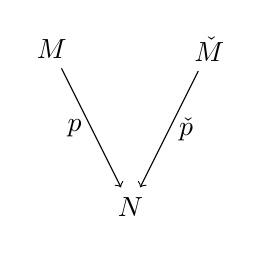
\begin{tikzpicture}
\draw (0,0) node (a) {$M$};
\draw (2,0) node (b) {$\check{M}$};
\draw (1,-2) node (c) {$N$};
\draw [->] (a) --node[left]{$p$} (c);
\draw [->] (b) --node[right]{$\check{p}$} (c);
\end{tikzpicture}
\end{figure}

Then \cite{SYZ} say $M$ and $\c{M}$ are mirror dual if they satisfy:
\begin{enumerate}[(i)]
\item For all regular points $x \in N$, $L_x\equiv p^{-1}(x)$ and
  $\check{L}_x\equiv \check{p}^{-1}(x)$ are \emph{special Lagrangian tori},
  i.e. $L$ is a torus, $\left.\omega\right|_{L}=0$ (Lagrangian) and
  $\left.\mbox{Im}(\Omega)\right|_{L}=0$ (special).
\item $L_x$ and $\check{L}_x$ are dual abelian varieties\footnote{Given
    $A$ an abelian variety over a field $k$, we define the functor
$\sP_A: \mbox{Sch}_{k} \rightarrow \mbox{Set}$ given by:
\[\sP_A(S) = \left\{\mbox{degree 0 line bundles } \sL \mbox{ over }A\times S \; | \;
\left.\sL\right|_{\{1\}\times S} \simeq \sO_S\right\},\]
where $1 \in A$ is the unit. A non-trivial important fact is that
$\sP_A$ is representable, the \emph{dual abelian variety} $\check{A}$ is
the representing object.}. In their formulation one actually requires
a weaker condition: that $L_x$ is a torsors for an abelian variety and
is in bijection with $\check{L}_x$ which is a torsor for the dual abelian
variety.
\end{enumerate}

\begin{rem*}
In general it is hard to produce special Lagrangian tori, however in
the case where $M$ comes from a Hyperk\"ahler manifold as explain in
the footnote any complex (for the $J_2$ structure) Lagrangian is
special. This will be the case for the Hitchin moduli spaces.
\end{rem*}

Before we focus on the example at hand, let's consider a slight
generalization of the above. One reference for this version of mirror
symmetry is also work of Hitchin \cite{H5}. In general
one might not have that the fibers of the above correspondence are
groups, but they might only be torsors for some abelian
variety $A$. Suppose that this abelian variety is $A \simeq
H^1(X,U(1))$ for some $X$, i.e. it is the Picard variety of some
curve. One wants to say that $L_x$ is a torsor for $H^1(X,U(1))$
geometrically. Note that if one has a trivial $U(1)$-bundle $L$ over
$X$, then the space of trivializations of $L$ is a
$H^0(X,U(1))$-torsor. This motivates one to consider a geometric
object over $X$, whose space of trivializations is a
$H^1(X,U(1))$-torsor.

\begin{defn}
Let $BU(1)$ be the sheaf\footnote{More precisely, $\sG$ over $X$ is a
  sheaf of categories (or groupoids) if for all $f: S \rightarrow X$ a cover,
  one has a data $f^*:\sG(X) \rightarrow \sG(S)$, and for $f^{(2)}:S^{(2)} \rightarrow
  S^{(1)}$ one has $\theta_{1,2}:f^{(2),*}\circ f^{(1),*} \rightarrow \left(f^{(1)}\circ
    f^{(2)}\right)^*$ satisfying:
\begin{enumerate}[(i)]
\item (\textit{presheaf}) $\theta_{1,23}\circ\theta_{2,3} = \theta_{12,3}\circ
  \theta_{1,2}$ for any chain of covers $S^{(3)}\overset{f^{(3)}}{\rightarrow}
  S^{(2)}\overset{f^{(2)}}{\rightarrow}S^{(1)}\overset{f^{(1)}}{\rightarrow}S \rightarrow X$;
\item (\textit{sheaf for morphisms}) For $X = \sqcup_{I}S_i$, then
  $g:P_1 \rightarrow P_2$ between two objects of $\sG(X)$ is specified by
  $g_i:\left.P_1\right|_{S_i}\rightarrow \left.P_2\right|_{S_i}$ for all $i$,
  such that $\left. g_i\right|_{S_{ij}} = \left.g_j\right|_{S_{ij}}$;
\item (\textit{sheaf for objects}) For $X = \sqcup_{I}S_i$, $Q_i \in
  \sG(S_i)$, with $u_{ij}:\left.Q_i\right|_{S_{ij}}\simeq
  \left.Q_i\right|_{S_{ij}}$ such that $u_{ij}u_{jk} = u_{ik}$, then
  there exists $Q \in \sG(X)$ glueing these objects.
\end{enumerate}
} of Picard
groupoids\footnote{A \emph{Picard groupoid} just means a groupoid
  which has a symmetric monoidal structure, where all objects are
  invertible, morally a group-object in the category of symmetric
  monoidal categories.} over $X$ given by: for every $U$ an open of
$X$
\[BU(1)(U) = \left\{U(1)\mbox{-torsors over }U\right\}.\]
A $U(1)$-\emph{gerbe} is a sheaf of Picard groupoids $\sA$ over $X$,
s.t. locally $\sA \simeq BU(1)$\footnote{One can continue to spell out
the details: $\sA$ is a gerbe for $A$ (a sheaf of groups on $X$) if it
is a sheaf of categories (we keep the same notation as before) and in
addition one has the conditions:
\begin{enumerate}[a.]
\item For all $i$, $Q_i \in \sA(S_1)$, $\mbox{Aut}(Q_i)$ is an
  $A$-torsor on $S_i$;
\item For all $Q_1,Q_2 \in \sA(S_1)$ there exists $\tilde{S}_1$,
  s.t. $\left.Q_1\right|_{\tilde{S}_1}\simeq
  \left.Q_2\right|_{\tilde{S}_1}$;
\item There exist a cover $\tilde{X} \rightarrow X$,
  s.t. $\sA(\tilde{X}) \neq \empty$.
\end{enumerate}}.
\end{defn}

\begin{rem*}
In the definitions in the footnotes we always think of \'etale
covers. We warn the reader that the notions of sheaf of categories,
groupoids, gerbes, etc. are very sensitive to the topology one uses.
\end{rem*}

We will note torture the reader with the definition of an isomorphism
between gerbes, see \cite{Br,DG} for details. The important take away
from it is the following two properties.

\begin{prop}
The isomorphism classes of $U(1)$-gerbes over $X$ are in bijection with
$H^2(X,U(1))$. Moreover, given $\sB$ a trivial $U(1)$-gerbe over $X$,
the space of trivializations of $\sB$, denoted
$\mbox{Triv}^{U(1)}(X,\sB)$ is a $H^1(X,\sB)$-torsor.
\end{prop}

Finally we reformulate the proposal of mirror symmetry as
follows. Suppose that in addition to the diagram above one also has
the data of $\sB$ a $U(1)$-gerbe over $M$ and $\check{\sB}$ a
$U(1)$-gerbe over $\check{M}$. Then, we say they are mirror dual to
each other if for all $x \in N$ regular:
\begin{enumerate}[(i)]
\item $L_x \simeq
  \mbox{Triv}^{U(1)}(\check{L}_x,\left.\check{\sB}\right|_{\check{L}_x})$;
\item $\check{L}_x \simeq
  \mbox{Triv}^{U(1)}(L_x,\left.\sB\right|_{L_x})$.
\end{enumerate}

\begin{rem*}
Note one needs to require both conditions, which was redundant before
since taking the double dual of an abelian variety is canonically
the identity.
Also, note that promoting the bijection of sets in the original
definition to a bijection of torsors is only a non-trivial statement
when made in families, in other words the use of gerbes is inevitable
in this situation.
This proposal was put forth first in \cite{H5} where he is trying to
make sense of what B-field are, i.e. the extra data of the gerbe
considered here.
\end{rem*}

\section{Hitchin moduli}

Fix a curve $X$ and $x_0 \in X$ a point. Let's recall that
\[M^d_{GL_r} = \left\{\mbox{stable degree d }GL_r-\mbox{principal
    bundles } E
  \mbox{ over }X \; | \; \psi \in H^0(X,\mbox{End}(E)\otimes
  K_X)\right\}\]
We first construct $M^d_{SL_r}$. Consider the map $\det: M^d_{GL_r}
\rightarrow M^d_{\mathbb{C}^{\times}}$ given by
\[\det((E,\psi)) = (\wedge^{r}E, \mbox{tr}\psi),\]
note that one obtains the trace of the Higgs field because one has to
consider the derivative of the determinant as the induced map on the
associated adjoint bundle. Let $(\sO_X(dx_0),0) \in
M^d_{\mathbb{C}^{\times}}$, then define $M^d_{SL_r}$ by the pullback diagram
\begin{figure}[h!]
\centering
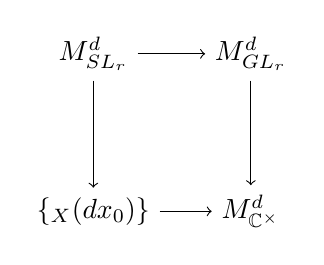
\begin{tikzpicture}
\draw (0,0) node (a) {$M^{d}_{SL_r}$};
\draw (2,0) node (b) {$M^{d}_{GL_r}$};
\draw (0,-2) node (c) {$\{\sO_X(dx_0)\}$};
\draw (2,-2) node (d) {$M^d_{\mathbb{C}^{\times}}$};
\draw [->] (a) -- (b);
\draw [->] (a) -- (c);
\draw [->] (c) -- (d);
\draw [->] (b) -- (d);
\end{tikzpicture}
\end{figure}

More concretely, one has $M^d_{SL_r}=\left\{(E,\psi) \in M^d_{GL_r} \;
  | \; \wedge^rE \simeq \sO_X(dx_0), \mbox{ and tr}(\psi) =
  0\right\}$.

Analogously for $M^d_{PGL_r}$. Recall that
\[1 \rightarrow \mu_r \rightarrow SL_r \rightarrow PGL_r \rightarrow 1\]
is an exact sequence which defines $PGL_r$. Let 
\[ \Gamma^r = \left\{\sL
\mbox{ degree 0 line bundle over }X \; | \; \sL^{\otimes r} =
\sO_X\right\},\] 
i.e. the $r$-torsion point of $\mbox{Pic}^0(X)$. Then
define $M^d_{PGL_r} = M^{d}_{SL_r}/\Gamma^r,$ where $\sL \in \Gamma^r$
acts by $(E,\psi) \mapsto (E\otimes \sL,\psi \otimes \sL)$.

We will denote by $B = \oplus^r_{i \geq 2}H^0(X,K^{\otimes i}_X)$ the
base of both Hitchin moduli, and by $\mu: M^d_{GL_r} \rightarrow B$ and
$\check{\mu}:M^d_{PGL_r} \rightarrow B$ the fibrations obtained by taking the
characteristic polynomials. Note that one does not have the first term
because of the traceless condition.

\begin{rem*}
For the reader that finds our construction of these moduli spaces
ad-hoc we remark that there is a general definition of these moduli
space for all reductive groups due to Simpson. It agrees with the one
took for $SL_r$ and $PGL_r$. The advantage of the one we adopted is
that one does not need to worry about what stability means for a
general principal $G$-bundle, which can be a little subtle.
\end{rem*}

Here is what we will prove in the next section. 
\begin{thm}
For any $(d,e) \in
\bZ\times \bZ$ there exist $U(1)$-gerbes $\sB^e$ over $M^d_{GL_r}$ and
$\check{\sB}^e$ over $M^e_{GL_r}$ such that they are mirror dual in the
generalized sense described in the last section.
\end{thm}

\begin{rem*}
Another prediction of mirror symmetry is a compatibility of the stringy
Hodge numbers. The paper \cite{HT} also has results in this direction
which we will not talk about here.
Note that $SL_r$ and $PGL_r$ are Langlands dual to each other. One can
ask if a similar duality holds in more generality, and that is true
and is the content of \cite{DP}.
\end{rem*}

\section{Universal families}

The title of this subsection is to involke what I believe is the
essential ingredient in the proof of the above result.

Henceforth $B$ will denote a Zariski open of the basis of the Hitchin,
defined by $x \in B$ such that the associated spectral curve
$\Sigma_x$ is smooth.

\textit{Step 1 (indentify the fibers):}
Recall that in $M^d_{GL_r}$ for a fixed
value of $x$, the characteristic polynomial, one has (cf. Lei's first
talk.):
\[\left\{(V,\psi) \; | \; \mbox{char}(\psi) = x\right\} \simeq
\left\{\sL \mbox{ a degree d line bundle over }\Sigma_x\right\}.\]
Now for $\mu^{-1}(x)$ one needs to consider $V$, s.t. $\wedge^rV
\simeq \sO_X(dx_0)$, that means $\sL \in \mbox{Pic}(\Sigma_x)^d$
s.t. $\wedge^r(\pi_*\sL) \simeq \sO_X(dx_0)$, where $\pi: \Sigma_x \rightarrow
X$. We denote it by $P^d\equiv \mu^{-1}(x)$. 

A similar analysis gives
that for $M^d_{PGL_r}$, one has $\check{\mu}^{-1} \equiv \check{P}^d =
P^d/\Gamma^r$, where the action of $\Gamma^r$ on $P^d$ is given by
$(L,\sL) \mapsto \pi^*L\otimes\sL$.

We note that in the same way that $\mbox{Pic}^d(\Sigma_x)$ is a
$\mbox{Pic}^0(\Sigma_x)$-torsor, $P^d$ and $\check{P}^d$ are $P^0$ and
$\check{P}^0$-torsors, respectively.

One also have that $P^0$ is dual (as an abelian variety) to
$\check{P}^0$. Indeed, consider the following exact sequence\footnote{We
  consider the exact sequence as groups, and $\mbox{Nm}$ is by
  definition $\mbox{det}\pi_*$ the norm map.}
\[1 \rightarrow P^0 \rightarrow \mbox{Pic}^0(\Sigma_x) \overset{\mbox{Nm}}{\rightarrow}
\mbox{Pic}^0(X) \rightarrow 1,\]
which one can dualize\footnote{Recall the Jacobians are self-dual
  abelian varieties.} to obtain
\[1 \rightarrow \mbox{Pic}^0(X) \rightarrow \mbox{Pic}^0(\Sigma_x) \rightarrow
\left(P^0\right)^{\vee} \rightarrow 1.\]
One just needs to prove the claim:
\[\left(P^0\right)^{\vee} \simeq \check{P}^0.\]
This follows from $\mbox{Pic}^0(\Sigma_x)\simeq
\left(\mbox{Pic}^0(X)\times P^0\right)/\Gamma^r$. Consider the functor
$\Phi: \mbox{Pic}^0(X)\times P^0 \rightarrow \mbox{Pic}^0(\Sigma_x)$ given by
\[\Phi(L,L') = \pi^*L^{-1}\otimes L'.\]
Then $\mbox{ker}(\Phi) = \{L' = \pi^*L\}$, so $\sO_X = \mbox{Nm}(L') =
\mbox{Nm}(\pi^*L)=L^{\otimes r}$, i.e. $L \in \Gamma^r$.

\textit{Step 2 (the gerbe $\sB$):}
Here is an important fact we will need in this step.
\begin{prop}
There exist an universal projective bundle $\sE$ over
$M^d_{SL_r}\times X$, i.e. for all $(V,\psi) \in M^d_{GL_r}$
\[\left.\sE\right|_{(V,\psi)\times X}\simeq P(V).\]
\end{prop}

\begin{rem*}
Similar statements are true for $GL_r$ or $PGL_r$ and the proof of
them comes from the construction of the moduli space, say $M$, of rank $r$
degree $d$ stable vector bundles over the curve $X$. Roughly speaking,
one can use the restriction on the
degree and rank to specify a certain Hilbert polynomial and consider
the corresponding connected component of the Quot scheme. Then one
knows that the Quot scheme has an universal sheaf by its very
construction. The subtle point is that to obtain $M$ one needs to
quotient the Quot scheme by isomorphisms of a quotient sheaf which give the
same vector bundle, this group of autormorphisms is $GL_r$. However, since by definition the
points of the Quot scheme are equivalence classes of maps $q: \sF \rightarrow
\sG$ with the same kernel one sees that the center $\mathbb{C}^{\times}$ acts
trivially on those points. Though, it does not act trivially on the
universal bundle, which is determined by $\sG$, i.e. $\sG$ gets
multiplied by a scalar. This implies that the GIT quotient used to
define $M$ will only have a universal \emph{projective} bundle,
i.e. defined up to multiplication by $\mathbb{C}^{\times}$. The interested
reader is refered to \cite[Chapter5]{Ne}, where this is beautifully
explained.
\end{rem*}

Let $\sF \equiv \left.\sE\right|_{M^d_{SL_r}\times \{x_0\}}$ be the
restriction of $\sE$ to the fiber at the point $x_0 \in X$. This is a
projective bundle over $M^d_{SL_r}$. We define for any $U \rightarrow
M^{d}_{SL_r}$ an \'etale map
\[\sB(U) \equiv \left\{\mbox{lifts of }\sF\mbox{ to a vector
    bundle}\right\}.\]
Here by vector bundle we mean a locally free sheaf over $U$.

\begin{lem}
$\sB$ is a $\mu_r$-gerbe over $M^d_{SL_r}$.
\end{lem}

\begin{proof}
Let $\sqcup_IS_i$ be an \'etale cover of $M^d_{SL_r}$. Consider $\sG
\in \sB(S_i)$. Let $\phi: \sG \rightarrow \sG$ be an automorphism, then for
$S_{ij}=S_i\times_{M^d_{SL_r}}S_j$ one has $\phi_j:
\left.\sG\right|_{S_{ij}}\rightarrow \left.\sG\right|_{S_{ij}}$ such that
$\left.\phi_j\right|_{S_{ijk}} =
\left.\phi_k\right|_{S_{ijk}}$. However this implies that $c_{ij}
\equiv \phi_j$ define a $GL_r$ cocycle on $S_i$. However one knows
that $\mathbb{P}(\phi_i) = \mbox{id}$\footnote{Here $\mathbb{P}(\sF)$ denotes the
  projectivization of the sheaf $\sF$.}, which implies $c_{ij} \in
H^0(S_{ij},\mathbb{C}^{\times})$. In other words, one gets $L_i$ a line
bundle on $S_i$ s.t. $\sG'\otimes L = \sG$ for another $\sG' \in
\sB(S_i)$. Since $\mathbb{P}(\sG')=\mathbb{P}(\sG\otimes L_i) = \sF$, one obtains
that $L_i \in \mbox{Pic}^0(M^d_{SL_r})[r]$, the $r$-torsion points of the
Jacobian variety of $M^d_{SL_r}$, because $\mathbb{P}(\sG\otimes L_i) =
\mathbb{P}(\sG)\otimes L^{\otimes r}_i$, since $\sG$ has rank $r$.
\end{proof}

\textit{Step 3 (triviality of $\sB$ restricted to $L_x$):}
We want to prove the fact that the gerbe constructed before is actually
trivial when restricted to $L_x$, the fiber of $\mu$. One needs to
check that any projective bundle $\sF$ over $L_x$ admits a lift to a
vector bundle.  Here is another important fact we will repeatedly use:
\begin{prop}
Given $N$ a moduli space of line bundles (e.g. fixed degree, fixed
norm, torsion, etc.) on a curve $Y$, and any element $L_0 \in
\mbox{Pic}(N)$, there exists an universal line bundle $\sL$ over $N\times Y$
s.t.
\[\left.\sL\right|_{N\times \{y\}} = L_0, \forall y \in Y, \; \mbox{and} \;
\left.\sL\right|_{\{n\}\times Y} = n \; \forall n \in N.\]
\end{prop}

\begin{rem*}
Notice this result is significantly different than the previous one
about the existence of projective universal families. Morally the
reason for this is that moduli spaces for line bundles are very
special.
\end{rem*}

Let $\tilde{\sL}$ be a universal line bundle over $P^d\times
\Sigma_x$, s.t. $\left.\mathbb{P}\left(\left(\mbox{id}\times
    \pi\right)_*(\tilde{\sL})\right)\right|_{P^d\times\{x_0\}} =
\left.\sF\right|_{P^d}$. Then $\left(\mbox{id}\times
  \pi\right)_*(\tilde{\sL})$ is a candidate for the lift of $\sF$ on
$P^d$. However, by picking a point $y \in \pi^{-1}(x_0)$ one can ask
that $\left.(\tilde{\sL})\right|_{P^d\times\{y\}} = L_0 \in
\mbox{Pic}^0(P^d)$ is a fixed element. Since one has
\[\det\left(\left(\mbox{id}\times\pi\right)_*(\tilde{\sL})\right) =
\otimes_{y \in \pi^{-1}(x)}\left.\tilde{\sL}\right|_{P^d\times\{y\}},\]
and there are $r$ of them because $\Sigma_x$ is an $r$-cover of
$X$. We let $L' \in \mbox{Pic}^0(P^d)$ be such that $L'^{\otimes r} =
\det\left(\left(\mbox{id}\times\pi\right)_*(\tilde{\sL})\right)$ and
taking $L_0 = \sO_{P^d}\otimes L'^{-1}$ we are done.

\textit{Step 4 ($U(1)$-trivializations):}
One is interested in $\mbox{Triv}^{\mu_r}(L_x,\sB)$, i.e. the
equivalence classes of trivializations of
$\left.\sB\right|_{L_x}$. This is a $H^1(L_x,\mu_r)$-torsor, i.e. a
$\mbox{Pic}^0(P^d)[r]$-torsor. 
One can look at this as a $\mbox{Pic}^0(P^d)$-torsor by
\[\mbox{Triv}^{U(1)}(L_x,\sB) \equiv
\mbox{Triv}^{\mu_r}(L_x,\sB)\times_{\mbox{Pic}^0(P^d)[r]}\mbox{Pic}^0(P^d).\]
Since $\sB$ is trivial, i.e. $\sB(L_x) \simeq \left\{\mu_r\mbox{-torsors on
  }L_x\right\}$, one can write $\mbox{Triv}^{U(1)}(L_x,\sB)$ as
\[\left\{\sL\mbox{ a universal line bundle over }P^d\times\Sigma_x \;
  | \; \left.\sL\right|_{P^d\times\{y\}}\in \mbox{Pic}^0(P^d) \;
  \forall y \in \Sigma_x\right\}.\]
This is exactly the construction we explained in Step 3.

Finally, to check the duality we need to prove the following:
\begin{lem}
\[\mbox{Triv}^{U(1)}(L_x,\sB) \simeq \check{P}^1.\]
\end{lem}

\begin{proof}
Recall $\check{P}^1 = \mbox{Pic}^1(\Sigma_x)/\mbox{Pic}^0(X)$ and
\begin{align*}
\mbox{Triv}^{U(1)}(L_X,\sB) = \left\{\sL\mbox{ is a universal line
    bundle over }\mbox{Pic}^d(\Sigma_x)\times\Sigma_x \; | \right. \\
\left. \left.\sL\right|_{\mbox{Pic}^d(\Sigma_x)\times\{y\}}\in\mbox{Pic}^0(\mbox{Pic}^d(\Sigma_x)),
  \; \forall y \in \Sigma_x\right\}/\mbox{Pic}^0(X),
\end{align*}
where $\mbox{Pic}^0(X)$ acts by the norm map. For convinience let's call the
righthand side above, before taking the quotient by $\mbox{Pic}^0(X)$,
by $\mathbb{L}$. So one is reduced to prove that
\[\mbox{Pic}^1(\Sigma_x) \simeq \mathbb{L}.\]
Let $y \in \Sigma_x$ and consider the element $T^1_y \in
\mbox{Pic}^1(\Sigma_x)$ given by $\sO_{\Sigma_x}(y)$ and let $T^2_y \in
\mathbb{L}$ be given by the universal line bundle $\sL$ on
$\mbox{Pic}^d(\Sigma_x)\times \Sigma_x$ s.t.
\[\left.\sL\right|_{\mbox{Pic}^d(\Sigma_x)\times\{y\}}=\sO_{\mbox{Pic}^d(\Sigma_x)}.\]
We just need to check that for all $y,y' \in \Sigma_x$, $T^1_{y'}-T^1_y
= T^2_{y'}-T^2_y$ as elements of $\mbox{Pic}^0(X)$. Indeed, $\sL \in T^2_y$ on
$\mbox{Pic}^d(\Sigma_x)\times \Sigma_x$ is defined as
$\pi^*_2L_0\otimes F_{L_0,y}^*\sP$ for $L_0 \in
\mbox{Pic}^d(\Sigma_x)$ and $F_{L_0,y}: \mbox{Pic}^d(\Sigma_x)\times
\Sigma_x \rightarrow \mbox{Pic}^0(\Sigma_x)\times \mbox{Pic}^0(\Sigma_x)$
given by $F_{L_0,y}(L,z) = (L\otimes L^{-1}_0,\sO_{\Sigma_x}(z-y))$,
here $\sP$ is the universal line bundle over the Jacobian, known as
the Poincar\'e bundle (see \cite[Chapter 16]{P} for details). It follows
that 
\[T^2_{y'}-T^2_y=\left(\pi^*_2L_0\otimes
  F^*_{L_0,y}\sP\right)\otimes\left(\pi^*_2L_0\otimes
  F^*_{L_0,y'}\sP\right)^{-1} = \sO_{\Sigma_x}(y'-y).\]
This concludes the proof of one of the dualities, the other is
completely analogous and we refer the reader to the original paper
\cite{HT} where it is carried out in details.
\end{proof}


% Matthew Talk 2
\chapter{Hitchin Systems and Supersymmetric Field Theories}

\section{Introduction and definitions}

In previous talks, we've explored many properties of the Hitchin system
and its geometry, as well as several applications. The core idea of
this talk is that, given a certain supersymmetric field theory, we
can obtain the Hitchin system as a moduli space associated to this
theory via a standard procedure in quantum field theories. Gaiotto,
Moore, and Neitzke \cite{GMN} use this approach to construct a canonical
coordinate system on the Hitchin moduli space. The goal of this talk
is to explain some of the language of supersymmetric quantum field
theories, and describe how we can obtain $\mathcal{M}_{H}$ from a
particular class of such theories.


\subsection{Supersymmetry}

Consider $\mathbb{R}^{n}$. The \textbf{Poincare group} is the group
of translations and rotations of this space: $G=ISO(n)\cong\mathbb{R}^{n}\rtimes SO(n)$.
(In Minkowski signature, say for $\mathbb{R}^{n,1}$, we might write
$ISO(n,1)$ instead). Recall that there's a spin group defined as
a double cover of $SO(n)$:
\[
\xymatrix{1\ar[r] & \mathbb{Z}_{2}\ar[r] & Spin(n)\ar[r] & SO(n)\ar[r] & 1.}
\]
When we have such a double cover, we get an extension of the group
$G$ to the supergroup $\tilde{G}$. This gives an extension of the
Poincare algebra $\mathfrak{g}$ to the \textbf{super Poincare algebra}
$\tilde{\mathfrak{g}}$ coming from the double-cover of $SO(n)$.
$\tilde{\mathfrak{g}}$ is called the \textbf{supersymmetry algebra}.
Such $\tilde{g}$ are labelled by a choice of a representation of
$Spin(n)$. For irreducible representations of $Spin(n)$, there are
two possible cases:
\begin{itemize}
\item There is either a unique irreducible spinor representation $S$, and
any spinor representation has the form $S^{\oplus N}$ for some $N$,
or
\item There are two distinct irreducible real spinor representations $S_{+},S_{-}$,
and any spinor representation has the form $S_{+}^{\oplus N_{1}}\oplus S_{-}^{\oplus N_{2}}$
for some $N_{1},N_{2}$. (This occurs in dimensions $n\equiv2,6\mod8$).
\end{itemize}
Thus, when someone says $N=n$ or $N=\left(n_{1},n_{2}\right)$ supersymmetry,
they are specifying which extension of the Poincare algebra they're
referring to.

The supersymmetry Lie algebra $\tilde{\mathfrak{g}}$ splits into
an even and odd part:
\[
\tilde{\mathfrak{g}}=\mathfrak{g}^{0}\oplus\mathfrak{g}^{1},
\]
and is equipped with a skew-symmetric bracket $\left[\cdot,\cdot\right]:\tilde{\mathfrak{g}}\rightarrow\tilde{\mathfrak{g}}$
which satisfies the Jacobi identity. Note that $\left[\mathfrak{g}^{1},\mathfrak{g}^{1}\right]\subset\mathfrak{g}^{0}$,
$\mathfrak{g}^{0}=\mathfrak{g}$ (the Poincare algebra), and $\mathfrak{g}^{1}$
is just a linear representation of $\mathfrak{g}^{0}$.
\begin{example*}
For $N=2$ SUSY and $G=ISO(3,1)$, we'll be interested in a $\tilde{G}$
whose Lie algebra has even part
\[
\mathfrak{g}^{0}=\mbox{\ensuremath{\mathfrak{iso}}}(3,1)\oplus\mathbb{C}.
\]
The abelian $\mathbb{C}$ factor is central in $\tilde{\mathfrak{g}}$,
and has a canonical generator $Z$.
\end{example*}

\subsection{BPS States}

Let $\mathcal{H}$ denote the Hilbert space of states of our quantum
system on $\mathbb{R}^{3,1}$. We want to think of a state as being
labeled by a representation of $\tilde{G}$---the representation encodes
the data of the particle. For example, the vacuum state (``empty
space'') in $\mathcal{H}$ corresponds to the trivial representation
of $\tilde{G}$. The next simplest kind of state is one where space
is empty except for a single particle propogating with some definite
momentum $p\in T^{*}\mathbb{R}^{3,1}$. Call the subspace of the Hilbert
space consisting of single-particle states $\mathcal{H}^{1}$. Here,
there's some structure:
\begin{itemize}
\item $\mathcal{H}^{1}$ splits into components $\mathcal{H}_{M}^{1}$,
labeled by $M\in\mathbb{R}_{\geq0}$. $M^{2}$ is the eigenvalue of
a quadratic Casimir operator in $ISO(3,1)$. Physically, it's the
mass of the particle.
\item For $N=2$ SUSY as in our prior example, we also have a central generator
$Z\in\mathbb{C}$. Together, these give a decomposition
\[
\mathcal{H}^{1}=\bigoplus_{M,Z}\mathcal{H}_{M,Z}^{1}.
\]

\end{itemize}
Fix some momentum $p_{rest}\in\left(\mathbb{R}^{3,1}\right)^{*}$
with $||p_{rest}||^{2}=M^{2}$, and consider the subspace $\mathcal{H}_{M,Z}^{1,rest}$
on which the subgroup of translations along $\mathbb{R}^{3,1}$ acts
by $p_{rest}$. This is a representation of a subgroup $\tilde{G}_{rest}\subset\tilde{G}$
with
\[
\tilde{G}_{rest}=SO\left(3\right)\ltimes\tilde{T},
\]
where the ``super translation group'' $\tilde{T}$ is generated
by the ordinary translations $T=\mathbb{R}^{3,1}$ plus the central
character $Z$ and the ``odd translations'' $\mathfrak{g}^{1}$.
The odd translations act by a Clifford algebra (on an 8-dimensional
vector space). We can then count the number of unitary irreducible
representations of this Clifford algebra:
\begin{itemize}
\item If $M<\left|Z\right|$, then there are \emph{no} unitary representations
of the Clifford algebra.
\item If $M=\left|Z\right|$, the Clifford algebra is degenerate, and its
unique unitary irrep $S$ has dimension $2^{4/2}=4$.
\item If $M>\left|Z\right|$, the Clifford algebra is nondegenerate, and
its unique unitary irrep $S$ has dimension $2^{8/2}=16$.
\end{itemize}
States that satisfy $M=\left|Z\right|$ are called \textbf{BPS} (Bogomol'nyi,
Prasad, Sommerfield) \textbf{states}, and as one might expect, they
satisfy a set of differential equations depending on the field theory.
The BPS states are those in which half of the supersymmetry generators
are unbroken.


\subsection{Moduli of Vacua}

The ``moduli space'' associated to a QFT typically refers to the
moduli space of vacua. By \textbf{vacua}, we mean the quantum state
with the lowest possible energy.
\begin{description}
\item [{Question}] In what sense is the space of vacua a moduli space?
\end{description}
For scalar fields, these are labelled by the \textbf{vacuum expectation
value} (VEV). The VEV of an operator is (as the name suggests) the
expectation value of the operator in the vacuum (the quantum state
with the lowest possible energy). We can label a vacuum state by its
VEV, and this gives a moduli space of vacua.

For $N=2$ SUSY, the superalgebra has two representations with scalars:
\textbf{vectormultiplets} (one complex scalar), and \textbf{hypermultiplets}
(two complex scalars). This gives a local splitting of the moduli
of vacua $\mathcal{M}$ as
\[
\mathcal{M}=\mathcal{M}_{C}\oplus\mathcal{M}_{H},
\]
where $\mathcal{M}_{C}$ is the ``Coulomb branch'' (vectormultiplets),
and $\mathcal{M}_{H}$ is the ``Higgs branch'' (hypermultiplets).


\section{Compactification and Dimensional Reduction}

Compactification of a field theory is a process where, instead of
considering a general space $X$, we consider $X=M\times C$ where
$C$ is some compact space. Dimensional reduction is the limit of
the compactified theory where the volume of the compact space is shrunk
to zero, which produces an effective theory on the remaining dimensions.
\begin{example*}
[Toy Example] Consider a field theory on $X=\mathbb{R}^{n}\times S_{R}^{1}$
($S_{R}^{1}$ is the circle of radius $R$). Let $\theta$ be a coordinate
on $S_{R}^{1}$, and $x^{i}$ coordinates on $\mathbb{R}^{n}$. At
a fixed $x$ coordinate, the fields along the $S_{R}^{1}$ look like
\[
\phi|_{x}=\sum_{n}A_{n}\cos\left(\frac{2\pi n}{R}\theta\right)+B_{n}\sin\left(\frac{2\pi n}{R}\theta\right),
\]
where the coefficients $A_{n}$ and $B_{n}$ are determined by the
boundary conditions on $\phi$. As $R\rightarrow0$, the eigenvalues
$\lambda_{n}=\frac{2\pi n}{R}$ approach $\infty$, except for $n=0$.
Note that in quantum mechanics, $\hbar\lambda_{n}$ is the \emph{momentum}
of eigenstate $n$, so as $R\rightarrow\infty$, all mometums except
the trivial one also $\rightarrow\infty$. We should interpert $R\rightarrow0$
as meaning that, for finite energy (and hence, finite momentum), the
only eigenstate left is the trivial one.

If $\phi|_{x}$ is constant, it means that the field $\phi$ does
not depend on $\theta$---the dimensional reduction of the theory
on $S_{R}^{1}$ consists of the fields of the $\mathbb{R}^{n}\times S_{R}^{1}$
theory which do not depend on $\theta$.
\end{example*}
So, we have two equivalent perspectives on dimensional reduction to
$M$ of a theory on a space $M\times C$:
\begin{itemize}
\item It's the limit of the theory on $M\times C$ where the volume of $C$
contracts to zero, or
\item It's the theory on $M\times C$ where all fields are taken to be independent
of coordinates on $C$.
\end{itemize}

\begin{example*}
[Yang-Mills] We actually already encountered dimensional reduction
in one of the first lectures of the course. Consider classical Yang-Mills
theory.

Yang-Mills theory is a field theory defined for principal $G$-bundles
$P\rightarrow X$, where $X$ is a 4-dimensional Riemannian manifold.
\begin{description}
\item [{Fields}] Connections $A$ on $P$.
\item [{Lagrangian}]
\[
L\left(A\right)=\left|F_{A}\right|^{2}d\mu
\]

\end{description}
Recall that from the Lagrangian, we obtain the action functional by
\[
S\left(A\right)=\int_{X}L\left(A\right)=\int_{X}\left|F_{A}\right|^{2}d\mu.
\]
The equations of motion for Yang-Mills theory are
\[
d_{A}^{*}F_{A}=0,
\]
and the instantons are the (anti) self-dual connections:
\[
F_{A}=\pm*F_{A}.
\]
(Here, $*:\Omega_{X}^{2}\cong\Omega_{X}^{2}$ is the Hodge star operator).

In local coordinates we can write $d_{A}=d+A$, where
\[
A=A_{1}dx_{1}+A_{2}dx_{2}+A_{3}dx_{3}+A_{4}dx_{4}.
\]
Define
\[
F_{ij}:=\left[\nabla_{i},\nabla_{j}\right]=\frac{\partial}{\partial x_{i}}A_{j}-\frac{\partial}{\partial x_{j}}A_{i}+\left[A_{i},A_{j}\right].
\]
Look at the self-dual connections. Then, the instanton equation $F_{A}^{-}=0$
becomes
\begin{eqnarray*}
F_{12} & = & F_{34},\\
F_{13} & = & -F_{24},\\
F_{14} & = & F_{23}.
\end{eqnarray*}


Let's restrict attention to $X=C\times\mathbb{R}^{2}$, where $C$
is a Riemann surface. Suppose that we compactify and perform dimensional
reduction in $\mathbb{R}^{2}$ coordinates: restrict to $A_{j}$ which
are invariant under translation in $x_{3}$, $x_{4}$. Then, $A_{1}dx_{1}+A_{2}dx_{2}$
defines a connection on $C$. Relabel $A_{3}=\phi_{1}$ and $A_{4}=\phi_{2}$,
and define $\varphi=\phi_{1}-i\phi_{2}$; then the self-dual equations
become
\begin{eqnarray*}
F_{A}-\frac{1}{2}i\left[\varphi,\varphi^{*}\right] & = & 0,\\
\left[\nabla_{1}+i\nabla_{2},\varphi\right] & = & 0.
\end{eqnarray*}
If we think of $\varphi$ as defining a local section of $\Omega^{0}\left(C;ad(P)\otimes\mathbb{C}\right)$,
and set $\Phi=\frac{1}{2}\varphi dz\in\Omega^{1,0}\left(ad\left(P\right)\otimes\mathbb{C}\right)$
and $\Phi^{*}=\frac{1}{2}\varphi^{*}d\overline{z}\in\Omega^{0,1}\left(ad(P)\otimes\mathbb{C}\right)$,
then the equations become
\begin{eqnarray*}
F_{A}+\left[\Phi,\Phi^{*}\right] & = & 0,\\
\overline{\partial_{A}}\Phi & = & 0,
\end{eqnarray*}
the usual Hitchin equations.
\end{example*}

\section{5D Super Yang-Mills Theory}

Now, let's repeat the previous example, but including some supersymmetry.
5D Super Yang-Mills theory admits a conventional Lagrangian description:
Let $P$ be a principal $G$-bundle over $X$ (a 5-dimensional space).
The theory has:
\begin{description}
\item [{Fields}] Connections $A$ on $P$, sections $\phi^{i}$ of $Ad\left(P\right)$
($i=1,\ldots,5$), and fermions.
\item [{Lagrangian}]
\[
L=\frac{R}{8\pi^{2}}Tr\left[\frac{1}{R^{2}}F_{A}\wedge*F_{A}+\sum_{i=1}^{5}d_{A}\phi^{i}\wedge*d_{A}\phi^{i}+\mbox{fermions}\right].
\]
\end{description}
\begin{rem*}
~
\begin{enumerate}
\item 5D SYM is well-defined as an effective field theory, below a certain
energy scale. It is not obviously well-defined at arbitrarily high
energies.
\item There's this unusual $R$ factor appearing here that you should be
suspicious of. We'll explain where this comes from at the end of the
talk.
\end{enumerate}
\end{rem*}

\subsection*{Compactification on $C$}

Let's take $X=\mathbb{R}^{2,1}\times C$, where $C$ is a Riemann
surface. Analogous to the classical case, when we compactify 5D SYM
on $C$, we combine $\phi^{4}$ and $\phi^{5}$ into a complex-valued
1-form on $C$:
\[
\varphi=\left(\phi^{4}+i\phi^{5}\right)dz.
\]
Note that to be a sensible theory, we additionally require translation 
invariance along $\mathbb{R}^{2,1}$.
\begin{description}
\item [{Question}] What are the classical field configurations in the compactified
theory which preserve the supersymmetry? (Recall that these are the
BPS states!)
\end{description}
Assuming $\phi^{1},\phi^{2},\phi^{3}=0$, the equations satisfied
by the remaining fields are
\[
\tag{\ensuremath{\star}}\begin{cases}
 & F_{A}+R^{2}\left[\varphi,\varphi^{*}\right]=0,\\
 & \overline{\partial_{A}}\varphi=0,
\end{cases}
\]
which we recognize as (almost) Hitchin's equations. In other words,
the moduli space of vacua of $SYM[C]$ in the low energy limit is
\[
M_{C}\left[G\right]=\left\{ \mbox{solutions to }(\star)\right\} /\left\{ \mbox{gauge transformations}\right\} =\mathcal{M}_{H}.
\]

\begin{rem*}
We took $\phi^{1}=\phi^{2}=\phi^{3}=0$ above. If we don't, SUSY also
imposes equations on $\phi^{1},\phi^{2},\phi^{3}$:
\begin{align*}
d_{A}\phi^{i} & =0, & \left[\varphi,\phi^{i}\right] & =0, & \left[\phi^{i},\phi^{j}\right] & =0.
\end{align*}
But, at a generic point in the moduli space, these equations won't
have any nontrivial solutions, so the assumption that $\phi^{j}=0$
isn't much of an imposition.
\end{rem*}

A key difference between this example and dimensional reduction for classical
Yang-Mills theory is that we have dimensionally reduced to a theory on $\mathbb{R}^{2,1}$,
\emph{not} a theory on $C$. Instead of seeing Hitchin's moduli space as the moduli of
instantons for our theory, it appears as the moduli of BPS states!

The full moduli space of vacua has a Coulomb branch---identified with
the Hitchin moduli space---and Higgs branches attached to the specific
other points where nontrivial solutions for the $\phi^{j}$ exist.
(Unfortunate nomenclature: the moduli of Higgs bundles is the space
of solutions that live on the Coulomb branch...)


\section{Compactification from (2,0) 6D Theory}

Now let's talk about where that pesky $R$ factor came from. It turns
out that there's a famous 6D $N=\left(2,0\right)$ QFT. It doesn't
have a conventional Lagrangian description (or even a space of fields).
Instead, the inputs are a 6-dimensional manifold, together with a
Lie algebra $\mathfrak{g}$. Call this theory $X_{\mathfrak{g}}$.
It has the following properties:
\begin{itemize}
\item $X_{\mathfrak{g}}$ has $N=\left(2,0\right)$ SUSY in $d=6$.
\item $X_{\mathfrak{g}}$ has no parameters---no coupling constants or scale,
and the strength of the interaction can't be perturbed.
\item $X_{\mathfrak{g}}$ is conformally invariant.
\end{itemize}
Despite its unconventional description, we can still compactify $X_{\mathfrak{g}}$
to obtain lower-dimensional theories. In fact, 5D SYM is $X_{\mathfrak{g}}\left[S^{1}\right]$,
where the $R$ is the length of the $S^{1}$. So, $\mathcal{M}_{H}$
is obtained as the moduli space associated to $X_{\mathfrak{g}}\left[C\times S^{1}\right]$.
We could perform this compactification in either order: $\mathcal{M}_{H}$
can also be obtained as the moduli space associated to the theory
$X_{\mathfrak{g}}\left[C\right]$ compactified on $S^{1}$. \cite{GMN}
use this observation to produce canonical Darboux coordinate systems
on $\mathcal{M}_{H}$ and construct Calabi-Yau metrics in these coordinate
systems.

Some examples of information we can obtain from this perspective:
\begin{itemize}
\item Compactify $X_{\mathfrak{g}}$ on $C$ first to get a 4d $N=2$ supersymmetric
gauge theory with with Coulomb branch $\mathcal{B}$. Then, $\mathcal{B}$
is actually the Hitchin base, i.e., $\mathcal{M}_{H}\rightarrow\mathcal{B}$
with generic fiber a torus. Points $u\in\mathcal{B}$ correspond to
spectral curves $\Sigma_{u}\subset T^{*}C$, also known as ``Seiberg-Witten
curves.''
\item $\mathcal{M}_{H}$ is automatically hyperkahler because of supersymmetry.
\end{itemize}

\input{17-Pyongwon-II.tex}

\input{18-Phil-II.tex}

\input{19-Lei-II.tex}

\input{20-Honghao-II.tex}

%% To add another chapter, create a new .tex file (e.g. 21-Peng-III.tex) and 
%% add the corresponding command: \input{21-Peng-III.tex}


%% Bibliography
\begin{thebibliography}{AB}
\bibitem[AB]{AB}M.~F.~Atiyah and R.~Bott, The Yang-Mills equations
over Riemann surfaces. Philos.~Trans.~Roy.~Soc. London A 308 (1982)
523--615.

\bibitem[B1]{B1}P.~Boalch, ``Geometry and Braiding of Stokes Data;
Fission and Wild Character Varieties,'' Annals of Math.~\textbf{179}
(2014) 301--365. http://annals.math.princeton.edu/wp-content/uploads/annals-v179-n1-p05-s.pdf

\bibitem[B2]{B2}P.~Boalch, ``Hyperkaehler Manifolds and Nonabelian
Hodge Theory of (Irregular) Curves,'' arXiv:1203.6607

\bibitem[BB]{BB}O.~Biquard and P.~Boalch. Wild non-abelian Hodge
theory on curves - 2004, Compos.~Math.~140 (2004) 179--204.

\bibitem[BNR]{BNR}A.~Beauville, M.~S.~Narasimhan, and S.~Ramanan,
``Spectral curves and the generalized theta divisor,'' J.~reine
angew.~Math. 398 (1989) 169--179 URL: http://math1.unice.fr/\textasciitilde{}beauvill/pubs/bnr.pdf

\bibitem[D]{D}S.~K.~Donaldson, ``A new proof of a theorem of Narasimhan
and Seshadri,'' J.~Differential Geometry, \textbf{18} (1983) 269--277.

\bibitem[DM]{DM}R.~Donagi and E.~Markman, ``Spectral covers, algebraically
completely integrable Hamiltonian systems, and moduli of bundles.''
arXiv:alg-geom/9507017

\bibitem[FG]{FG}V.~Fock and A.~Goncharov, Moduli spaces of local
systems and higher Teichmueller theory, Publ. Math. Inst. Hautes Etudes
Sci. No. 103 (2006), 1\textendash{}211.

\bibitem[GMN]{GMN} D.~Giaotto, G.~Moore, and A.~Neitzke, Wall-crossing,
Hitchin systems, and the WKB approximation. arXiv:0907.3987

\bibitem[H1]{H1}N.~Hitchin, ``The self-duality equations on a Riemann
surface,'' Proc. Long. Math. Soc. 55 (1987) 59--126.

\bibitem[H2]{H2}N.~Hitchin, ``Stable bundles and integrable systems,''
Duke Math J. 54 (1987) 91--114.

\bibitem[H3]{H3}N.~Hitchin, ``Lie Groups and Teichmueller Space,''
Topology 31 (1992) 449--473.

\bibitem[HT]{HT}T.~Hausel and M.~Thaddeus. Mirror symmetry, Langlands
duality, and the Hitchin system. Invent. Math., 153 (1):197\textendash{}229,
2003.

\bibitem[KW]{KW}A.~Kapustin and E.~Witten, ``Electric-Magnetic
Duality and the Geometric Langlands Program,'' CNTP 1 (2007()1--236.
arXiv:hep-th/0604151

\bibitem[N]{N}A.~Neitzke, ``Hitchin systems in N=2 field theory,''
https://www.ma.utexas.edu/users/neitzke/expos/hitchin-systems.pdf

\bibitem[NS]{NS}M.~S.~Narasimhan and C.~S.~Seshadri, `Stable
and unitary vector bundles on a compact Riemann surface,' Ann.~of
Math.~\textbf{82} (1965) 540--567.

\bibitem[W]{W}E.~Witten, ``Gauge Theory and Wild Ramification,''
arXiv:0710.0631\end{thebibliography}

\end{document}
